\section{Implementierung} \label{sec:Implementierung}

\subsection{Quantenalgorithmus}
Wie im Kapitel~\ref{Funktionsweise} zur Funktionsweise erklärt,
wird für die Periodenbestimmung die Quantum-Phase-Estimation genutzt.

Um den Quantum-Phase-Estimation Algorithmus für die Periodenberechnung zu nutzen,
benötigt man ein \(U\)-Gatter, 
welches die modulare Multiplikation, 
als eine unitäre Transformation realisiert:
\[U^{\tensor n}\ket{x}_n=\ket{a y \bmod N}_n\]
Mit dem passenden \(U\)-Gatter wird der Quantenschaltkreis wie in Abbildung~\ref{fig:shor_n_qubit} strukturiert.
\begin{figure}
    \centering
    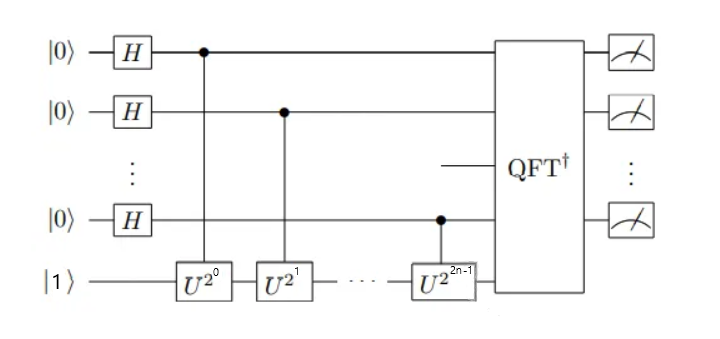
\includegraphics[width=\columnwidth]{shor_n_qubit.png}
    \caption{QPE für Shor~\cite{anonymousket}}
    \label{fig:shor_n_qubit}
  \end{figure}

Die Realisierung der Transformation erfordert die Implementierung einiger arithmetischer Operationen in Quantenschaltkreisform. 
Diese fungieren als Bausteine, die zusammengesetzt zur Konstruktion des übergeordneten Quantenschaltkreises für die modulare Multiplikation beitragen. 
Zu den erforderlichen arithmetischen Operationen gehört die Addition, Subtraktion sowie die modulare Addition.

In den folgenden Abschnitten werden die untergeordneten arithmetischen Operationen bis hin zur modularen Multiplikation implementiert.

\subsubsection{Addition} \label{sec:QuantumAdder}
Der Quantenschaltkreis für die Addition bildet das Fundament der \(U\)-Gatter und 
stellt einen der am häufigsten verwendeten Bausteine dar. 
Deswegen hat die Implementierung der Addition einen erheblichen Einfluss auf den Ressourcenbedarf des gesamten Quantenalgorithmus
und sollte daher möglichst effizient umgesetzt werden.

Eine Möglichkeit, die Addition als Quantenschaltkreis zu realisieren, 
besteht im Nachbau eines klassischen Schaltkreises aus Volladierern. 
Da es nicht möglich ist, 
die notwendigen klassischen Gatter wie AND und OR als unitäre Transformation mit nur zwei Qubits darzustellen~\cite{Hoever2023QC},
werden zusätzliche Hilfsqubits benötigt.
Die zusätzlichen Hilfsqubits bewirken, dass der Nachbau eines klassischen Schaltkreises für die Addition zweier \(n\)-Bit Zahlen, 
also solche der Größenordnung \(2^n\), mindestens \(3n\) Qubits benötigt~\cite{zalka1998fast}.

Eine effizientere Methode, welche ohne Hilfsqubits auskommt, ist die Quanten"=Addition~\cite{draper2000addition}. 
Die Quanten-Addition führt die Berechnung auf quantenmechanische Weise durch. 
Im Wesentlichen wird dabei die Addition in der Fourierbasis berechnet. 
Dafür befindet sich ein Summand des Quantenregisters \(\ket{b}_n\) in der Standardbasis und 
der andere Summand des Quantenregisters \(\ket{a}_n\) in der Fourierbasis.
Da sich das zweite Quantenregister in der Fourierbasis \(\Phi\) befindet, 
wird dieses als \(\ket{\Phi(a)}_n\) bezeichnet.
Anschließend kontrolliert der Summand in \(\ket{b}_n\) kontrollierte Phasen-Gatter, 
die auf den anderen Summanden in \(\ket{\Phi(a)}_n\) wirken.
Die durch die kontrollierten Phasen-Gatter induzierten Phasenverschiebungen übertragen die Werte, 
die dem Zustand des Summanden \(\ket{b}_n\) in der Fourierbasis entsprechen.
Dadurch befindet sich anschließend in dem Zielregister der Phasen-Gatter die Addition beider Werte in der Fourierbasis mit \(\ket{\Phi(a+b)}_n\).

Im Folgenden wird ein Beispiel für die Quanten-Addition zweier Quantenregister \(\ket{a}_3\) und \(\ket{b}_3\) betrachtet:
\begin{figure}[H]
    \centering
    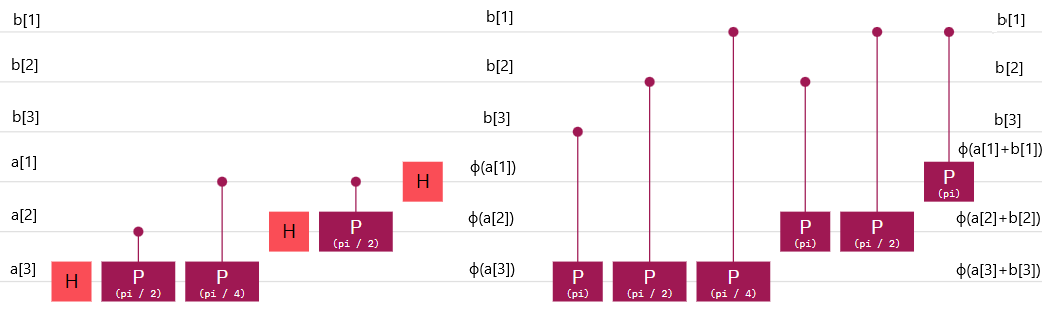
\includegraphics[width=\columnwidth]{3_qubit_quantum_add.png}
    \caption{Quantum-Addition}
    \label{fig:3_qubit_quantum_add}
  \end{figure}
Die Registermarkierungen in der Mitte von Abbildung~\ref{fig:3_qubit_quantum_add} unterteilen die Darstellung in zwei Hälften.
Die linke Hälfte repräsentiert die Quanten-Fourier-Transformation, 
während die rechte Hälfte die Quanten-Addition zeigt.

Wie man an der Struktur der Quanten-Addition erkennen kann,
ist die Anordnung der Gatter fast identisch mit der Quanten-Fourier-Transformation.
Ein Unterschied besteht darin, 
dass die Hadamard-Gatter durch kontrollierte \(P(\pi)\) Phasen-Gatter ersetzt wurden.
Sowohl das Hadamard-Gatter als auch das \(P(\pi)\) Phasen-Gatter erzeugt eine relative Phase von \(e^{\pi i}\).
Ein weiterer Unterschied zur Quanten-Fourier-Transformation besteht darin, 
dass die kontrollierten Phasen-Gatter nicht durch das Quantenregister kontrolliert werden, 
auf das die Gatter auch wirken.
Stattdessen kontrollieren die Qubits des Quantenregisters \(\ket{b}_3\) die Phasen-Gatter, 
welche auf das \(\ket{a}_3\) Quantenregister wirken.
Dabei wird das \(P(\pi)\) Phasen-Gatter durch das Qubit, des Quantenregisters \(\ket{b}_3\) kontrolliert,
welches die gleiche Wertigkeit hat wie das Zielqubit des Quantenregisters \(\ket{a}_3\).
Jedes weitere kontrollierte Phasen-Gatter für das gleiche Zielqubit 
wird fortlaufend von dem nächstkleineren Qubit des Quantenregisters \(\ket{b}_3\) kontrolliert.

Im Prinzip handelt es sich bei dieser Quantenschaltung um eine Anwendung derselben Phasenverschiebungen 
wie bei der Quanten-Fourier-Transformation. 
Der grundlegende Unterschied liegt darin, 
dass diese Phasenverschiebungen kontrolliert auf ein anderes Quantenregister angewendet werden.

Die Wirkung der Quanten-Addition wird anhand der Abbildung~\ref{fig:3_qubit_quantum_add} verdeutlicht.
Zu Beginn der linken Hälfte befinden sich beide Quantenregister in der Standardbasis.
Auf das Zielregister \(\ket{a}_3\) wird die Quanten-Fourier-Transformation ohne Swap-Gatter angewendet.
Dadurch befindet sich \(\ket{a}_3\) nun in der Fourierbasis \(\Phi\), also \(\ket{\Phi(a)}_3\):
\begin{align*}
  \begin{aligned}
  &\ket{\Phi(a)}_3 =\\
  &\frac{1}{\sqrt{8}} \Bigg[ \Big(\ket{0} + { e^{\frac{2 \pi i (2^0a_1)}{2^1}}}\ket{1} \Big) \tensor
  \Big(\ket{0} + { e^{\frac{2 \pi i (2^1a_2+2^0a_1)}{2^2}}}\ket{1} \Big) \tensor
  \Big(\ket{0} + { e^{\frac{2 \pi i (2^{2}a_3 +2^1a_2+2^0a_1)}{2^3}}}\ket{1} \Big) \Bigg]
  \end{aligned}
\end{align*}
Anschließend wird auf das hinterste Tensorprodukt ein \(P(\pi)\) Phasen-Gatter angewendet,
das von \(\ket{b_3}_1\) kontrolliert wird.
Wenn sich Qubit \(\ket{b_3}_1\) im Zustand \(\ket{0}\) befindet, passiert nichts.
Befindet es sich jedoch im Zustand \(\ket{1}\), wird die Phasenverschiebung des Phasen-Gatters angewendet.
Dieses Verhalten lässt sich für beide Fälle mit den entsprechenden Matrizen
\begin{align*}
  \begin{pmatrix}
    1 & 0 \\
    0 & e^{\pi i b_3}
  \end{pmatrix}  
  \text{beziehungsweise}  
  \begin{pmatrix}
    1 & 0 \\
    0 & e^{\frac{2\pi i (2^2b_3)}{2^3}}
  \end{pmatrix}
\end{align*}
beschreiben.
Schreibt man das hinterste Tensorprodukt als Vektor, ergibt sich die folgende Formulierung:
\[\frac{1}{\sqrt{2}}( \ket{0} + { e^{\frac{2 \pi i (2^{2}a_3 +2^1a_2+2^0a_1)}{2^3}}}\ket{1}) =
\frac{1}{\sqrt{2}}
\begin{pmatrix}
     1  \\
     e^{\frac{2 \pi i (2^{2}a_3 +2^1a_2+2^0a_1)}{2^3}}
  \end{pmatrix}
    \]
Dann wird durch das Ergebnis der Verrechnung mit dem Phasen-Gatter deutlich, 
dass die Addition im Wesentlichen in der Phase des Quantenzustands stattfindet:
\[\begin{pmatrix}
    1 & 0 \\
    0 & e^{\frac{2\pi i (2^2b_3)}{2^3}}
  \end{pmatrix}
    \cdot
\frac{1}{\sqrt{2}}
\begin{pmatrix}
    1  \\
     e^{\frac{2 \pi i (2^{2}a_3 +2^1a_2+2^0a_1)}{2^3}}
  \end{pmatrix}
  =
  \frac{1}{\sqrt{2}}
  \begin{pmatrix}
    1  \\
     e^{\frac{2 \pi i (2^{2}(a_3+b_3) +2^1a_2+2^0a_1)}{2^3}}
  \end{pmatrix}
\]
Wie in der Abbildung~\ref{fig:3_qubit_quantum_add} erkenntlich,
wirken auf das hinterste Tensorprodukt auch noch die beiden Phasen-Gatter \(P(\frac{\pi}{2})\) und \(P(\frac{\pi}{4})\) mit:
\begin{align*}
    P(\frac{\pi}{2}) &= 
\begin{pmatrix}
    1 & 0 \\
    0 & e^{\frac{\pi}{2} i b_2}
  \end{pmatrix}
  =
  \begin{pmatrix}
    1 & 0 \\
    0 & e^{\frac{2\pi i (2^1b_2)}{2^3}}
  \end{pmatrix} \\
P(\frac{\pi}{4}) &= 
\begin{pmatrix}
    1 & 0 \\
    0 & e^{\frac{\pi}{4} i b_1}
  \end{pmatrix}
  =
  \begin{pmatrix}
    1 & 0 \\
    0 & e^{\frac{2\pi i (2^0b_1)}{2^3}}
  \end{pmatrix}
\end{align*}
Multipliziert man beide von links an das vorherige Ergebnis erhält man:
\begin{align*}
    &\begin{pmatrix}
        1 & 0 \\
        0 & e^{\frac{2\pi i (2^0b_1)}{2^3}}
      \end{pmatrix}
      \cdot
      \begin{pmatrix}
        1 & 0 \\
        0 & e^{\frac{2\pi i (2^1b_2)}{2^3}}
      \end{pmatrix}
      \cdot
      \frac{1}{\sqrt{2}}
      \begin{pmatrix}
        1  \\
         e^{\frac{2 \pi i (2^{2}(a_3+b_3) +2^1a_2+2^0a_1)}{2^3}} 
      \end{pmatrix} 
     \\
      =&
      \frac{1}{\sqrt{2}}
      \begin{pmatrix}
        1  \\
         e^{\frac{2 \pi i (2^{2}(a_3+b_3) +2^1(a_2+b_2)+2^0(a_1+b_1))}{2^3}}
      \end{pmatrix}
\end{align*}
Wendet man alle weiteren Phasen-Gatter auf das vollständige Tensorprodukt an, 
wird dies zu:
\begin{align*}
    \frac{1}{\sqrt{8}} 
    \Bigg[ 
      \Big(\ket{0} + { e^{\frac{2 \pi i (2^0(a_1+b_1))}{2^1}}}\ket{1} \Big) 
      \tensor
      \Big( &\ket{0} + { e^{\frac{2 \pi i (2^1(a_2+b_2)+2^0(a_1+b_1))}{2^2}}}\ket{1} \Big)\\ 
      &\tensor
      \Big( \ket{0} + { e^{\frac{2 \pi i (2^{2}(a_3+b_3) +2^1(a_2+b_2)+2^0(a_1+b_1))}{2^3}}}\ket{1} \Big) 
    \Bigg]
\end{align*}
Setzt man in diese Formel zwei Zahlen in Binärschreibweise ein, 
wird man denselben Zustand erhalten,
als würde man die Summe der beiden Zahlen in die Formel der Quanten-Fourier-Transformation einsetzt.
Beispielsweise sei \(a = 3\) also binär \(a_3 = 0\), \(a_2 = 1\),\(a_1 = 1\) und 
\(b = 1\) also \(b_3 = 0\), \(b_2 = 0\),\(b_1 = 1\):
\begin{align*}
\frac{1}{\sqrt{8}} 
\Bigg[ \Big(\ket{0} + { e^{\frac{2 \pi i (2^0(1+1))}{2^1}}}\ket{1} \Big) 
\tensor
\Big( \ket{0} + &{ e^{\frac{2 \pi i (2^1(1+0)+2^0(1+1))}{2^2}}}\ket{1} \Big) \\
&\tensor
\Big( \ket{0} + { e^{\frac{2 \pi i (2^{2}(0+0) +2^1(1+0)+2^0(1+1))}{2^3}}}\ket{1} \Big) 
\Bigg]
\end{align*}
\[
=\frac{1}{\sqrt{8}} 
\Bigg[ \Big(\ket{0} + \ket{1} \Big) \tensor
\Big( \ket{0} +   \ket{1} \Big) \tensor
\Big( \ket{0} +  e^{\pi i }\ket{1} \Big) 
\Bigg]
\]
Dass dies tatsächlich der Summe in der Fourierbasis entspricht, wird deutlich, 
wenn man das gleiche Tensorprodukt im Kontext der Quanten-Fourier-Transformation bildet:
\begin{align*}
    QFT(\ket{c}_3) = 
    \frac{1}{\sqrt{8}} 
    \Bigg[ \Big(\ket{0} + { e^{\frac{2 \pi i (2^0(c_1))}{2^1}}}\ket{1} \Big) 
    \tensor
    \Big( \ket{0} + &{ e^{\frac{2 \pi i (2^1(c_2)+2^0(c_1))}{2^2}}}\ket{1} \Big) \\
    &\tensor
    \Big( \ket{0} + { e^{\frac{2 \pi i (2^{2}(c_3) +2^1(c_2)+2^0(c_1))}{2^3}}}\ket{1} \Big) 
\Bigg]
\end{align*}
Die Summe von \(a\) und \(b\) entspricht \(c = 4\) also \(c_3 = 1,~c_2 = 0,~c_1=0\):
\begin{align*}
    QFT(\ket{4}_3) &=
    \begin{aligned}[t]
      \frac{1}{\sqrt{8}} \Bigg[ \Big(\ket{0} + { e^{\frac{2 \pi i (2^0(0))}{2^1}}}\ket{1} \Big) 
      &\tensor
      \Big( \ket{0} + { e^{\frac{2 \pi i (2^1(0)+2^0(0))}{2^2}}}\ket{1} \Big) \\
      &\tensor
      \Big( \ket{0} + { e^{\frac{2 \pi i (2^{2}(1) +2^1(0)+2^0(0))}{2^3}}}\ket{1} \Big) \Bigg]
    \end{aligned} \\
    &= 
    \frac{1}{\sqrt{8}} \Bigg[ \Big(\ket{0} + { e^{\frac{2 \pi i (0)}{2^1}}}\ket{1} \Big) 
    \tensor
    \Big( \ket{0} + { e^{\frac{2 \pi i (0)}{2^2}}}\ket{1} \Big) 
    \tensor
    \Big( \ket{0} + { e^{\frac{2 \pi i (2^{2}(1))}{2^3}}}\ket{1} \Big) \Bigg] \\
    &=\frac{1}{\sqrt{8}} \Bigg[ \Big(\ket{0} + \ket{1} \Big) 
    \tensor
    \Big( \ket{0} +   \ket{1} \Big) 
    \tensor
    \Big( \ket{0} +  e^{\pi i }\ket{1} \Big) \Bigg]
\end{align*}
Der Zustand, 
der durch die Quanten-Addition der Summanden \(a=3\) und 
\(b=1\) in zwei verschiedenen Quantenregistern mit jeweils drei Qubits erzeugt wird, 
entspricht dem Zustand, der entsteht, 
wenn man die Quanten-Fourier-Transformation auf ein Quantenregister mit drei Qubits anwendet, 
das die Summe der beiden Zahlen enthält.

Mit einer anschließenden inversen Quanten-Fourier-Transformation 
kann die Summe in die Standardbasis und somit in einen messbaren Zustand transformiert werden:
\[
iQFT(\ket{\Phi(4)_3})
=
 iQFT \Bigg(\frac{1}{\sqrt{8}} \Big[ (\ket{0} + \ket{1} ) \tensor
( \ket{0} +   \ket{1} ) \tensor
( \ket{0} +  e^{\pi i }\ket{1} ) \Big]\Bigg) 
=
\ket{4}_3
\]

Das Zielregister sollte aus genügend Qubits bestehen, 
damit die Summe vollständig erfasst werden kann.
Andernfalls kommt es zum Overflow mit \(a + b \bmod 2^n\), 
wobei \(n\) die Anzahl der Qubits des Zielregisters beschreibt.

Für die Realisierung der modularen Multiplikation wird zu keinem Zeitpunkt der Berechnung eine Addition zweier Zwischenergebnisse benötigt. 
Genauer gesagt, ist es nicht nötig, ein Quantenregister auf ein anderes zu addieren. 
Stattdessen wird die Quanten-Addition benutzt, um eine vorab bekannte Zahl auf ein Quantenregister zu addieren.

Bei der Quanten-Addition mit zwei Quantenregistern, 
wie in Abbildung~\ref{fig:3_qubit_quantum_add} erfolgt die Phasenverschiebung kontrolliert,  
also in Abhängigkeit des Inhaltes von Quantenregister \(\ket{b}_3\).
Ist der Inhalt von Quantenregister \(\ket{b}_3\) vorab bekannt,
können gewöhnliche Phasen-Gatter anstelle von kontrollierten verwendet werden~\cite{beauregard2003circuit}.

Wenn bei der Quanten-Addition mit zwei Quantenregistern ein Phasen-Gatter aufgrund des zugehörigen Kontrollqubits im Zustand \(\ket{1}\) angewendet wird,
wird es in der Variante mit einem einzelnen Quantenregister als gewöhnliches Phasen-Gatter verwendet.
Ist das Kontrollqubit hingegen im Zustand \(\ket{0}\), 
wodurch das Phasen-Gatter bei der Quanten-Addition mit zwei Quantenregistern nicht zur Anwendung kommt, 
wird dieses Phasen-Gatter in der Variante mit nur einem Quantenregister weggelassen.

\begin{figure}[H]
  \centering
  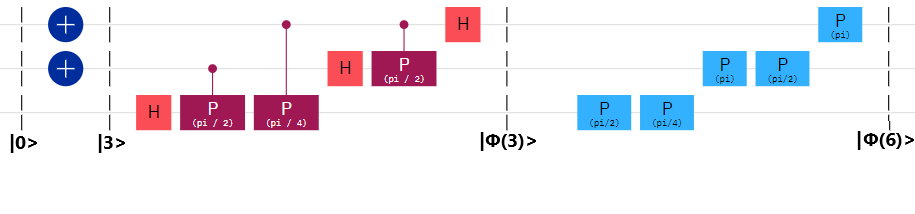
\includegraphics[width=\columnwidth]{3_qubit_fixed_quantum_addition.png}
  \caption{Quantum-Addition fixierte Phasenverschiebungen}
  \label{fig:3_qubit_fixed_quantum_addition}
\end{figure}
In Abbildung~\ref{fig:3_qubit_fixed_quantum_addition} ist die Quanten-Addition für ein 3-Qubit Quantenregister abgebildet.
Die blauen Phasen-Gatter sorgen für die Quanten-Addition mit einem fixierten Wert von \(3\).
Vergleicht man Abbildung~\ref{fig:3_qubit_fixed_quantum_addition} mit Abbildung~\ref{fig:3_qubit_quantum_add} fällt auf, 
dass das allererste Phasen-Gatter der Quanten-Addition nicht vorkommt.
Im Quantenschaltkreis der Abbildung~\ref{fig:3_qubit_quantum_add} würde ein Registerinhalt von \(b = 3\) das Kontrollqubit \(b_3\) nicht setzen. 
Somit kommt das erste Phasen-Gatter der Quanten-Addition nicht zum Einsatz und 
wird deswegen in der Variante wie in Abbildung~\ref{fig:3_qubit_fixed_quantum_addition} weggelassen. 

Des Weiteren ist es möglich, 
den Quantenschaltkreis der Quanten-Addition für eine vorab festgelegte Zahl ressourcensparender zu realisieren.
Die Optimierung bezieht sich dabei auf die Anzahl der verwendeten Gatter.
Wird die Quanten-Addition für eine feste Zahl realisiert, 
können für jedes einzelne Qubit die angewendeten Phasenverschiebungen vorab zusammengerechnet werden.
Demnach bietet es sich an, 
die zusammengerechneten Phasenverschiebungen in ein einzelnes Phasen-Gatter zusammenzufassen.
Nach diesem Prinzip benötigt man für eine Quanten-Addition maximal ein einzelnes Phasen-Gatter pro Qubit.

\begin{figure}[H]
  \centering
  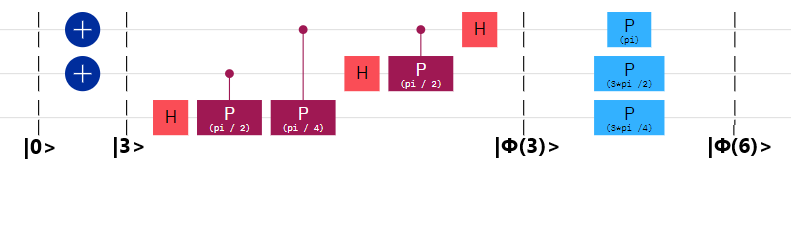
\includegraphics[width=\columnwidth]{3_qubit_fixed_quantum_addition_opt.png}
  \caption{Ressourcensparende Quantum-Addition}
  \label{fig:3_qubit_fixed_quantum_addition_opt}
\end{figure}
Der Quantenschaltkreis in Abbildung~\ref{fig:3_qubit_fixed_quantum_addition_opt} führt die identische 
Berechnung durch wie der Quantenschaltkreis aus Abbildung~\ref{fig:3_qubit_fixed_quantum_addition}.
Darüber hinaus werden die benötigten Phasenverschiebungen mit einem einzigen Phasen-Gatter pro Qubit realisiert.

Die Implementierung nutzt die ressourceneffiziente Variante der Quanten-Addition.
In der Funktion \texttt{A\_Gate} wird ein Gatter erzeugt, 
das sämtliche für die Quanten-Addition erforderlichen Phasen-Gatter umfasst.
Der Code zur Funktion ist in Abbildung~\ref{code:QuantumAdd} dargestellt.
\begin{listing}[H]
\begin{minted}[linenos,fontsize=\footnotesize]{python}    
def A_Gate(a_bin: list[int]) -> qiskit.circuit.gate:
    A_Gate = qiskit.QuantumCircuit(len(a_bin))
    theta_list = [0.0]*len(a_bin)
    for target_bit in range(len(a_bin)):
        exponent = 1
        for control_bit in reversed(range(target_bit+1)):
            if a_bin[control_bit] == 1:
                theta_list[target_bit]+= 2*pi/(2**(exponent))
            exponent+=1
    for qubit_index in range(len(a_bin)):
        A_Gate.append(P_Gate(theta_list[qubit_index]),[qubit_index])
    A_Gate = A_Gate.to_gate()
    A_Gate.name = " Add(" + str (binToDez(a_bin) )+ ")"
    return A_Gate 
  \end{minted}
  \caption{Quantum-Addition in Qiskit}
  \label{code:QuantumAdd}
\end{listing}
Der Funktion \texttt{A\_Gate} wird der zu addierende Summand im Binärformat übergeben, 
wobei am Index Null das Least-Significant-Bit liegt.
Abhängig von der Anzahl der Bits des Summanden wird ein Quantenschaltkreis mit der gleichen Anzahl an Qubits erzeugt. 
In den Zeilen 4 bis 9 werden die Phasenverschiebungen, die auf ein einzelnes Qubit wirken sollen, berechnet und akkumuliert.
Anschließend wird in den Zeilen 10 bis 11 auf jedes Qubit des Quantenschaltkreises ein individuelles Phasen-Gatter angewendet.
Die Phasenverschiebung eines einzelnen Phasen-Gatters ergibt sich aus der vorherigen Akkumulation in den Zeilen 4 bis 9.
Abschließend wird der Quantenschaltkreis in ein Gatter umgewandelt und mit einer passenden Bezeichnung versehen.

\subsubsection{Subtraktion}
Die Quanten-Addition besteht ausschließlich aus unitären Gattern und ist daher selbst ebenfalls unitär.
Diese Eigenschaft vereinfacht die Implementierung der Subtraktion. 
Durch die Invertierung der Quanten-Addition ergibt sich ein Quantenschaltkreis, 
der eine Subtraktion in der Fourierbasis ausführt. 
Damit erhält man praktisch einen Quantenschaltkreis, für die Quanten-Subtraktion.

Genau wie bei der Quanten-Addition kann es auch bei der Quanten-Subtraktion zu einem Overflow
oder im konkreten Kontext zu einem Underflow kommen.
Dieser Effekt tritt ein, 
falls der im Zielregister befindliche Minuend kleiner ist als der Subtrahend.

Der Effekt des Underflows wird verwendet, um herauszufinden, 
ob der Subtrahend größer als der Minuend ist.
Angenommen, man hat zwei Zahlen, 
die maximal der Größenordnung \(2^n\) entsprechen und 
ein Zielregister, 
welches aus \(n+1\) Qubits besteht.
Der Minuend \(b\) befindet sich im Zielregister, 
also \(\ket{\phi(b)}_{n+1}\), 
worauf die Quanten-Subtraktion mit dem Subtrahenden \(a\) wirkt.
Dann existieren zwei mögliche Fälle~\cite{beauregard2003circuit}:
\[b \geq a~\rightarrow~\ket{\phi(b-a)}_{n+1};~
b < a~\rightarrow~\ket{\phi(2^{n+1}-(a-b))}_{n+1}
  \]
Das Most-Significant Bit ist ausschließlich im zweiten Fall gesetzt und kann somit, 
nachdem das Quantenregister in die Standardbasis transformiert wurde, 
als eine Art Borrow-Bit verwendet werden.

Die Implementierung der Quanten-Subtraktion ist aufgrund der \texttt{inverse} Funktion von Qiskit unkompliziert.
Wendet man die \texttt{inverse} Funktion auf ein Gatter der Quanten-Addition aus der \texttt{A\_Gate} Funktion an, 
wird dieses in die Quanten-Subtraktion invertiert.
Der zugehörige Code ist in~\ref{code:QuantumSub} abgebildet.
\begin{listing}[H]
\begin{minted}[linenos,fontsize=\footnotesize]{python}    
def S_Gate(subtrahend_bin: list[int]) -> qiskit.circuit.gate:
    S_Gate = A_Gate(subtrahend_bin).inverse()
    S_Gate.name = "  Sub(" + str (binToDez(subtrahend_bin) )+ ")"
    return S_Gate
  \end{minted}
  \caption{Quantum-Subtraktion in Qiskit}
  \label{code:QuantumSub}
\end{listing}

\subsubsection{Modulare Addition} \label{sub:modulareAddition}
Das Gatter der Quanten-Addition und der Quanten-Subtraktion ermöglichen die Konstruktion einer unitären Transformation, 
welche die Berechnung der modularen Addition realisiert.
Gemeinsam bilden sie einen Quantenschaltkreis, 
der das Ergebnis der Berechnung \(\ket{\Phi(a+b)\bmod N}\) für \(a, b < N\) im Zielregister speichert.

\begin{figure}[H]
  \centering
  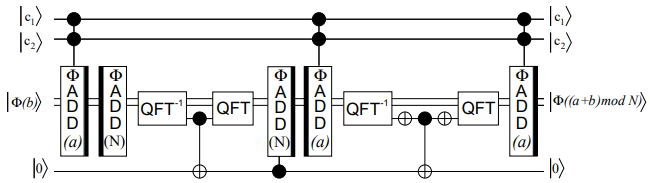
\includegraphics[width=\columnwidth]{Modular_adder_Paper.PNG}
  \caption{Modulare Addition nach Beauregard~\cite{beauregard2003circuit}}
  \label{fig:modulare_addition_paper}
\end{figure}
Abbildung~\ref{fig:modulare_addition_paper} zeigt das Konzept, 
das als Bauplan für die Implementierung der modularen Addition diente.
In der Grafik sind zwei Arten von \(\phi ADD\)-Gattern zu sehen:
Die Quanten-Addition, erkennbar an dem fettgedruckten Strich auf der rechten Seite 
und die Quanten-Subtraktion, erkennbar an dem fettgedruckten Strich auf der linken Seite.
Sowohl die Quanten-Addition als auch die Quanten-Subtraktion addieren beziehungsweise subtrahieren eine feste Zahl und 
sind somit die zuvor vorgestellten Varianten mit gewöhnlichen Phasen-Gattern.

Der Quantenschaltkreis zur modularen Addition agiert als Baustein in einem größeren Gesamtbild. 
Aus diesem Grund werden zwei Kontrollqubits \(\ket{c_1}_1\) und \(\ket{c_2}_1\) eingebaut, 
die im weiteren Verlauf Anwendung finden.
Das Eingaberegister, das zugleich als Zielregister dient,  
ist initial bereits in der Fourierbasis mit \(\ket{\phi(b)}\).

Das Zielregister wird um ein weiteres Qubit erweitert, 
welches das Most-Significant-Bit des Zielregisters darstellt.
Dieses Qubit hat einen besonderen Anwendungszweck und wird im Weiteren als Borrow-Qubit bezeichnet.
Insgesamt besteht das Zielregister also aus \(n+1\) Qubits, 
wenn der Modulus \(N\) einer Größenordnung von \(2^n\) entspricht.
Alle nachhaltigen Veränderungen durch den Quantenschaltkreis betreffen ausschließlich das Zielregister.
Darüber hinaus verwendet die Quantenschaltung ein weiteres Qubit, 
welches initial im Zustand \(\ket{0}\) ist.
Der Zustand dieses einzelnen Qubits bedingt eine Fallunterscheidung in der Berechnung des Quantenschaltkreises und 
wird daher im Weiteren als Bedingungs-Qubit bezeichnet. 

Um die Berechnung des Quantenschaltkreises nachvollziehen zu können, 
werden die Auswirkungen der verwendeten Gatter im Einzelnen erklärt.
Die erste Quanten-Addition sorgt dafür, 
dass auf das initiale Zielregister \(\ket{\phi(b)}\) eine Addition mit \(a\) angewendet wird und 
dadurch \(\ket{\phi(b + a)}\) entspricht.
Darauf folgt eine Quanten-Subtraktion, 
die mit dem Subtrahend \(N\) auf das Zielregister \(\ket{\phi(b + a)}\) wirkt und 
dieses in den Zustand \(\ket{\phi(b + a - N)}\) überführt. 
Daraus resultieren zwei mögliche Zustände:
\[1.~(b+a) \geq N~\rightarrow~\ket{\phi((b+a) - N)}_{n+1}\]
\[2.~
(b+a) < N~\rightarrow~\ket{\phi(2^{n+1}-(N-(a+b)))}_{n+1}
  \]
Im ersten Fall entspricht das Ergebnis der korrekten Berechnung von \(a+b \bmod N\).
In diesem Fall ist der Inhalt des Quantenregisters mit \(a+b \bmod N\) kleiner als \(N\), 
weshalb das Borrow-Bit nicht gesetzt ist.
Im Gegensatz dazu ist das Ergebnis im zweiten Fall fehlerhaft.
Da bei \((b+a) < N\) bereits der Rest der modularen Restklasse im Register steht, 
wird durch die Quanten-Subtraktion ein \(N\) zu viel vom Registerinhalt abgezogen.
Dadurch entsteht ein Underflow im Zielregister, 
wodurch das Borrow-Bit gesetzt wird.

Als Nächstes wirkt die inverse Quanten-Fourier-Transformation auf das Zielregister und 
führt eine Transformation in die Standardbasis durch.
Aufgrund des Basiswechsels in die Standardbasis beschreiben die Zustände der Qubits des Zielregisters nun das Ergebnis in der Binärdarstellung.
Im ersten Fall befindet sich das Borrow-Bit im Zustand \(\ket{0}\) und im zweiten Fall im Zustand \(\ket{1}\).
Anhand dieser Unterscheidung kann man eine bedingte Operation mittels eines kontrollierten X-Gatters realisieren.
Dafür kontrolliert das Borrow-Bit ein X-Gatter, 
welches auf das Bedingungs-Qubit wirkt.
Dadurch wird das Bedingungs-Qubit ausschließlich im zweiten Fall in den Zustand \(\ket{1}\) versetzt.
Danach wird das Zielregister wieder in die Fourierbasis transformiert, 
indem die Quanten-Fourier-Transformation angewendet wird.
Anschließend kontrolliert das Bedingungs-Qubit eine Quanten-Addition mit dem Summanden \(N\) auf das Zielregister.
Die kontrollierte Quanten-Addition wird also nur im zweiten Fall angewendet und korrigiert das vorher ungültige Ergebnis
zu dem korrekten:
\[
\ket{\phi(2^{n+1}-(N-(a+b)))}_{n+1} \underrightarrow{~+N~} 
\ket{\phi(2^{n+1}+(a+b))}_{n+1} \underrightarrow{\text{overflow }2^{n+1}}
\ket{\phi(a+b)}_{n+1}
  \]
Nun befindet sich in beiden Fällen das korrekt berechnete Ergebnis im Zielregister mit \(\ket{\Phi(a+b)\bmod N}\).
Somit ist die Berechnung der modularen Addition abgeschlossen.

Je nachdem, welcher der beiden Fälle eingetreten ist, 
befindet sich das Bedingungs-Qubit in einem anderen Zustand.
Um zu verhindern, dass sich das Bedingungs-Qubit in einem ungewissen Zustand befindet und dadurch zum "`Trash"'-Qubit wird, 
wird der initiale Zustand \(\ket{0}\) des Bedingungs-Qubit durch die restlichen Gatter des Quantenschaltkreises wiederhergestellt.
Ein eindeutiger Zustand ermöglicht, dass das Bedingungs-Qubit bei weiteren Berechnungen wiederverwendet werden kann.

Um das Bedingungs-Qubit zurückzusetzen, 
wird zuerst eine Quanten-Subtraktion mit \(a\) auf das Zielregister angewendet.
Um die Auswirkungen dieser Quanten-Subtraktion hervorzuheben, wird der Registerinhalt für beide Fälle untersucht:
Im ersten Fall war \((b+a) \geq N\) weswegen die Subtraktion von \(N\) zum Ergebnis der modularen Addition führte.
Da \(a, b < N\) gilt, ist das Ergebnis der modularen Addition kleiner als \(a\).
Die Quanten-Subtraktion mit \(a\) führt also zu einem Underflow, wodurch das Borrow-Bit gesetzt wird.
Im zweiten Fall war \((b+a) < N\).
Deswegen wurde die Subtraktion von \(N\) nicht durchgeführt, 
beziehungsweise wieder rückgängig gemacht, da \((b+a)\) bereits das Ergebnis der modularen Addition ist.
Für den zweiten Fall gilt als Ergebnis also \((b+a)\).
Dies ist nicht kleiner als \(a\), 
darum kommt es zu keinem Underflow und das Borrow-Bit wird deswegen nicht gesetzt.
Der Zustand des Borrow-Bits ist nun also im Vergleich zu den Fällen des vorherigen Abschnitts der Quantenschaltung invertiert.

Um das Borrow-Bit auslesen zu können, 
wird analog zum vorherigen Abschnitt des Quantenschaltkreises eine inverse Quanten-Fourier-Transformation durchgeführt.
Anschließend wird ein X-Gatter auf das Borrow-Bit angewendet.
Dadurch befindet sich das Borrow-Bit nun in denselben Zuständen wie in den beiden Fällen des ersten Abschnitts der Quantenschaltung.
Im nächsten Schritt kontrolliert das Borrow-Bit ein X-Gatter, das auf das Bedingungs-Qubit wirkt.
Dadurch wird es wieder in den initialen Zustand \(\ket{0}\) versetzt.

Um den Zustand \(\ket{\Phi(a+b)\bmod N}\) des Zielregisters wiederherzustellen, 
werden die Gatter bis zur Quanten-Subtraktion mit \(a\)
nun in umgekehrter Reihenfolge und invers angewendet.
Zunächst wird ein selbstinverses X-Gatter auf das Borrow-Bit angewendet.
Danach folgt die Quanten-Fourier-Transformation, 
die quasi die Inverse der inversen Quanten-Fourier-Transformation darstellt.
Abschließend folgt die Quanten-Addition mit \(a\), 
um die zuvor erfolgte Quanten-Subtraktion von \(a\) auf das Zielregister zu revertieren.

Das Zielregister beinhaltet nun den gewünschten Zustand:
\[\ket{\Phi(a+b)\bmod N} \text{ für } a, b < N\]
Des Weiteren befindet sich das Bedingungs-Qubit wieder im initialen Zustand \(\ket{0}\) und kann für weitere Rechnungen wiederverwendet werden.

\bigskip

Wenn man den Quantenschaltkreis in Abbildung~\ref{fig:modulare_addition_paper} betrachtet,
fällt auf, 
dass nicht alle Quanten-Additionen und Quanten-Subtraktionen kontrolliert durchgeführt werden.
Die modulare Addition soll nur dann ausgeführt werden, 
wenn die Kontrollqubits \(\ket{c_1}_1\) und \(\ket{c_2}_1\) gesetzt sind.

Betrachtet man ausschließlich die kombinierte Wirkung der Gatter des Quantenschaltkreises, 
welche nicht von \(\ket{c_1}\) und \(\ket{c_2}\) kontrolliert sind, 
führen diese lediglich die Identitätstransformation durch~\cite{beauregard2003circuit}.
Dies liegt daran, dass keine modulare Addition mit \(a\) durchgeführt werden soll, 
wenn \(\ket{c_1}\) oder \(\ket{c_2}\) im Zustand \(\ket{0}\) ist. 
Aufgrund der Bedingung \(b < N\), 
steht bereits der modulare Rest im Zielregister und somit ist keine Berechnung notwendig.

Der Grund, weshalb nicht alle Quanten-Additionen, 
Quanten-Subtraktionen und gegebenenfalls sogar die (inversen) Quanten-Fourier-Transformationen kontrolliert sind,
liegt in der erhöhten Komplexität, die dadurch im Quantenschaltkreis entstehen würde~\cite{beauregard2003circuit}.
Wenn ein Kontrollqubit nicht aktiviert ist, wird das kontrollierte Gatter trotzdem ausgeführt, jedoch ohne praktische Wirkung.
Abbildung~\ref{fig:gatedef_U1U2U3_CNOT} zeigt die physikalische Implementierung dreier Single-Qubit-Gatter im Vergleich zu einem kontrollierten X-Gatter.
Wie in der Abbildung erkennbar, 
benötigt das kontrollierte Gatter mehr Hardware-Elemente als die drei Single-Qubit-Gatter.
Somit ist es nicht möglich, 
die Komplexität des Quantenschaltkreises zu verringern, 
indem zusätzliche Gatter kontrolliert angewendet werden.

\begin{figure}[H]
  \centering
  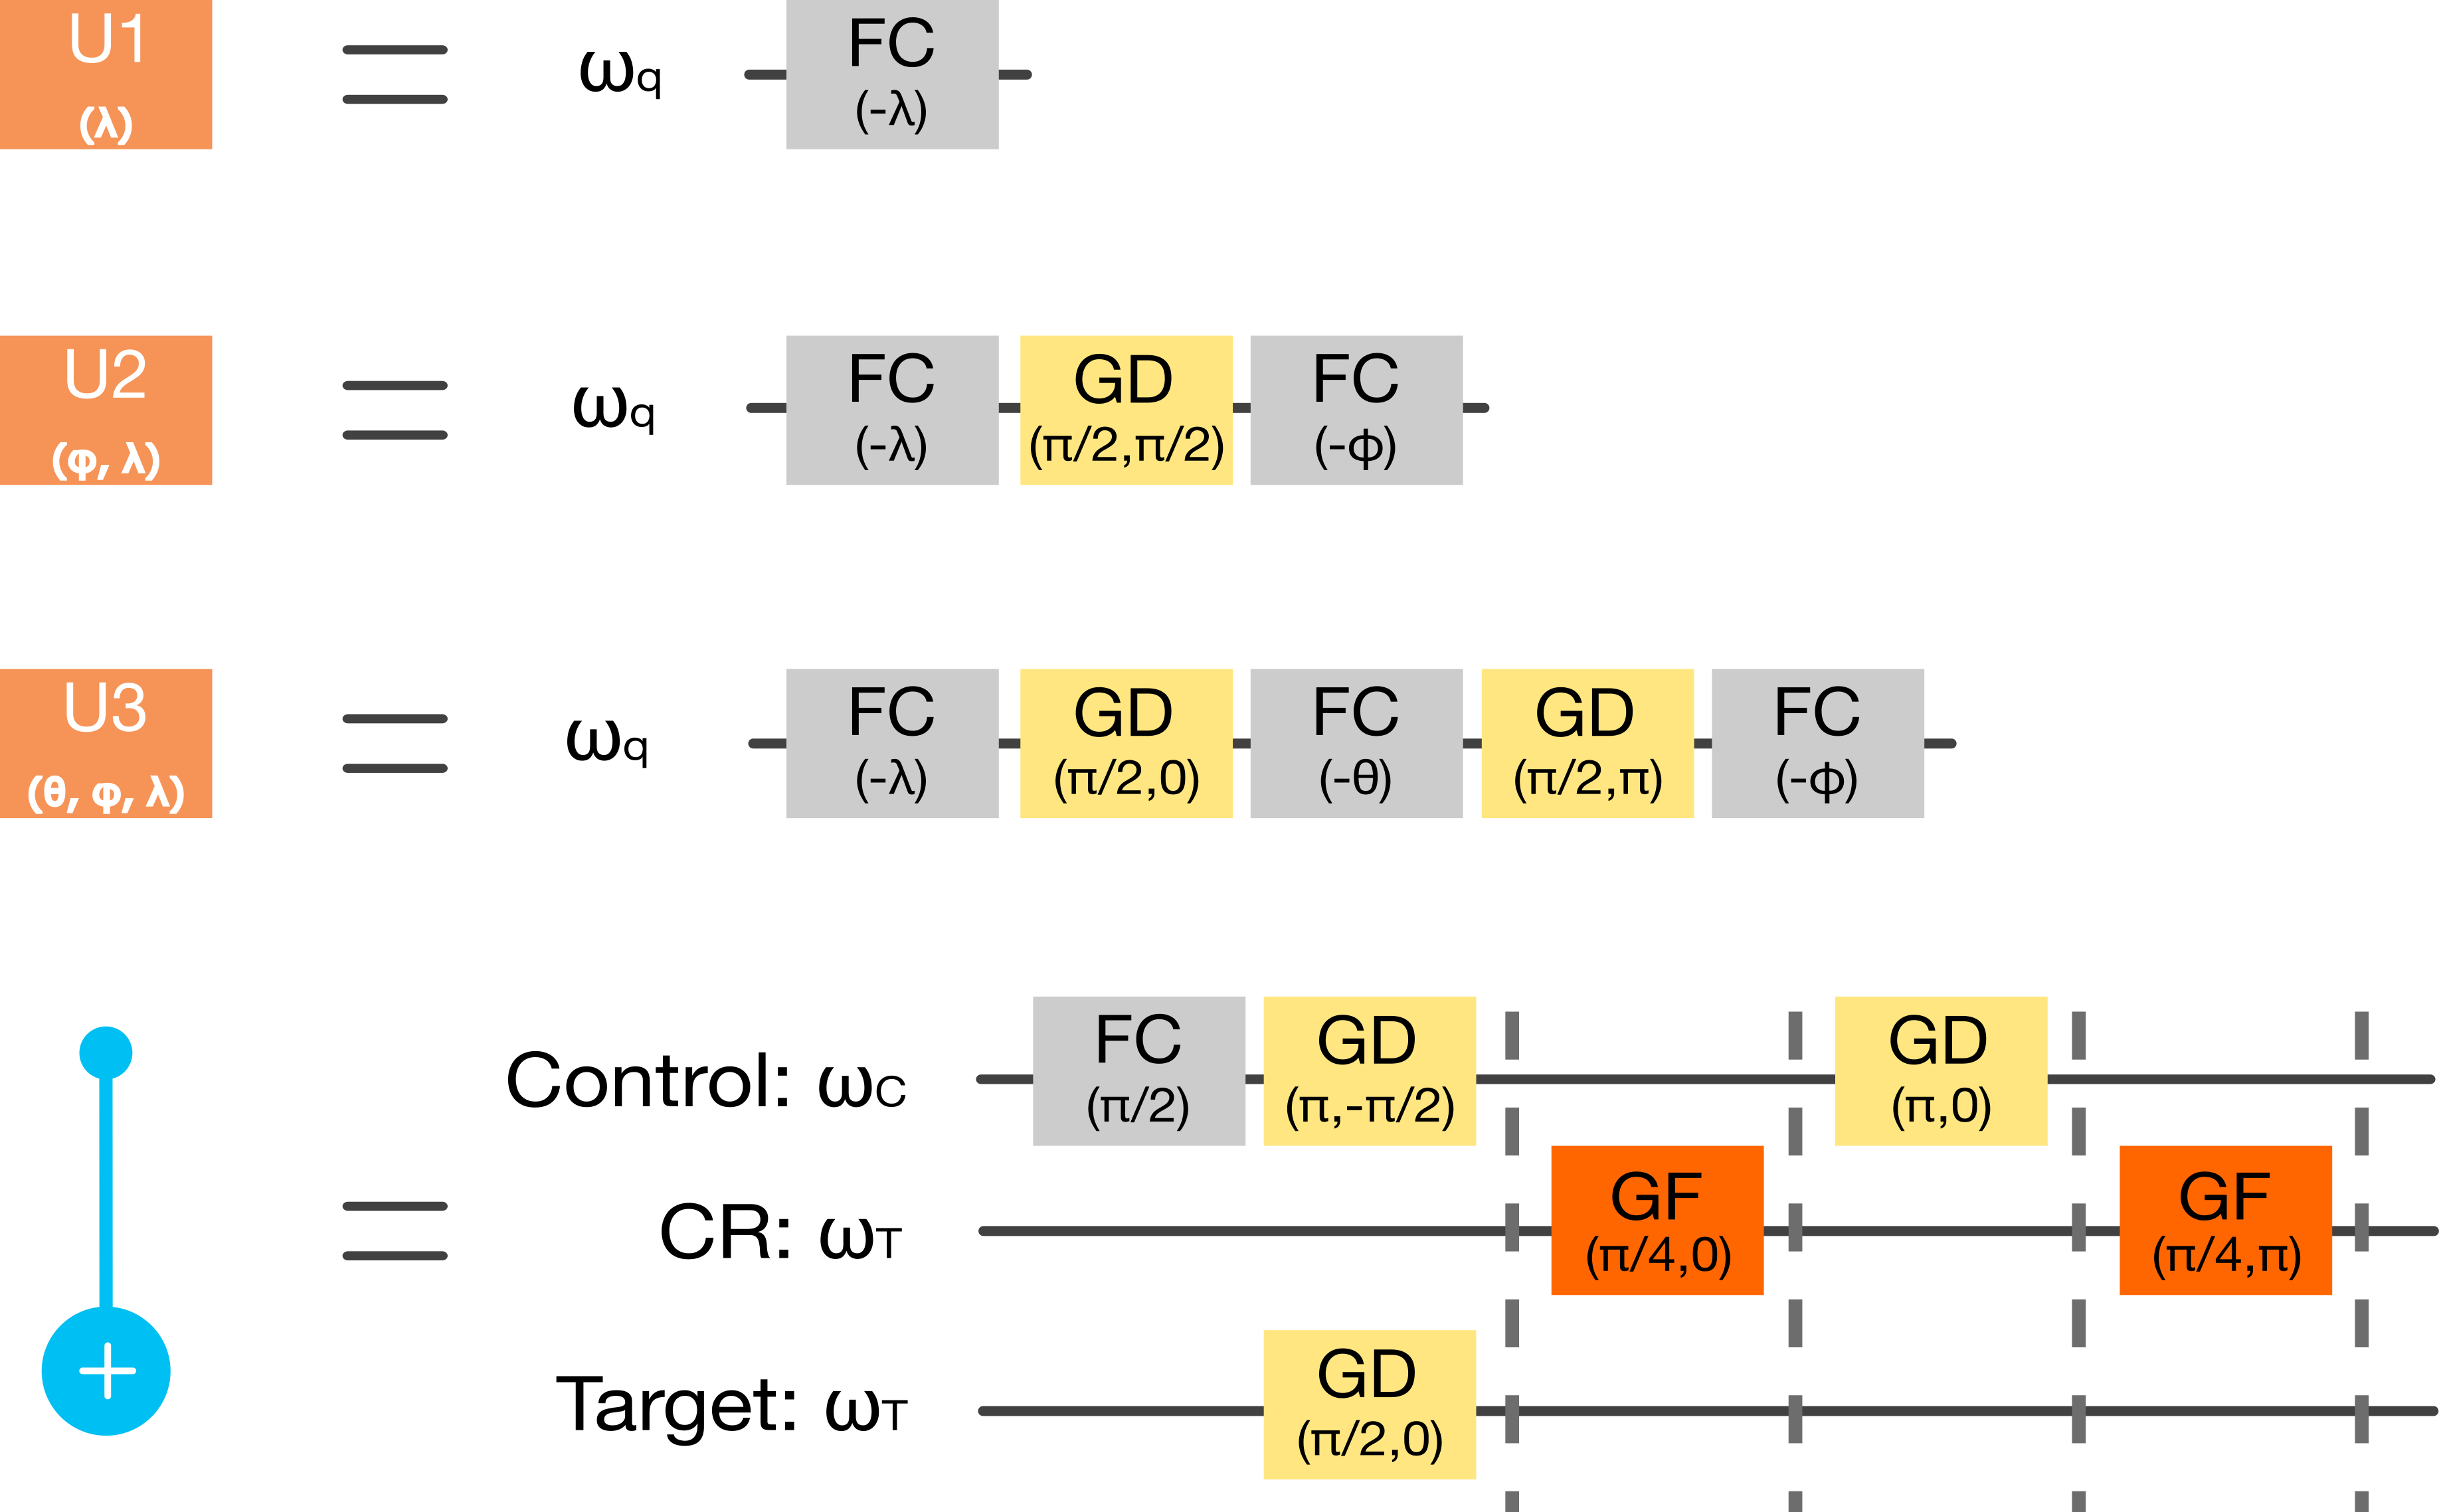
\includegraphics[scale=0.5]{gatedef_U1U2U3_CNOT.png}
  \caption{Physikalische Implementierung~\cite{ibmqx5}}
  \label{fig:gatedef_U1U2U3_CNOT}
\end{figure}

Ein weiterer Aspekt, 
der die Komplexität der Quantenschaltung für die modulare Addition erhöht, 
ist der Abschnitt, der das Bedingungs-Qubit zurücksetzt.
Wäre es möglich, diesen Teil auszulassen, könnten zwei der insgesamt fünf Quanten-Additionen bzw. 
Quanten-Subtraktionen sowie die Hälfte der (inversen) Quanten-Fourier-Transformationen eingespart werden.

Es gibt die Möglichkeit, bei einem Qubit einen Reset durchzuführen, wodurch dieses den Zustand \(\ket{0}\) annimmt.
In Qiskit kann dies mit der Funktion \texttt{Reset} realisiert werden~\cite{qiskitReset}.
Die Verwendung ist jedoch nicht zielführend, da diese durch keine unitäre Abbildungsmatrix
beschrieben werden kann.
Somit ist die Reset-Transformation nicht unitär und würde deswegen dazu führen, dass alle Quantenalgorithmen, 
die diese Funktion nutzen, ebenfalls nicht mehr unitär wären.
Da die Quantum-Phase-Estimation den Eigenwert einer \textit{unitären} Transformation extrahiert, 
ist diese Funktion für die Anwendung im Shor-Algorithmus ungeeignet.

\begin{figure}[H]
  \centering
  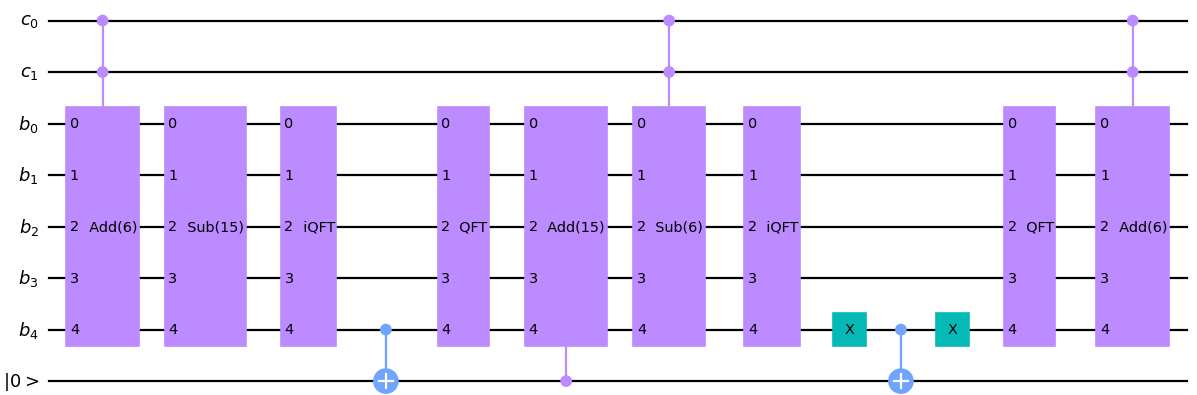
\includegraphics[width=\columnwidth]{modulareAddition.png}
  \caption{Qiskit modulare Addition}
  \label{fig:ModularAddition}
\end{figure}

Abbildung~\ref{fig:ModularAddition} zeigt die Implementierung eines Gatters für die modulare Addition 
mit \(a = 6\) und \(N = 15\) in Qiskit.
Der zugehörige Code, der ein Gatter wie in Abbildung~\ref{fig:ModularAddition} generiert, 
ist in der Funktion \texttt{Modular\_Adder\_Gate}~\ref{code:ModularAddition} enthalten.

Die Funktion \texttt{Modular\_Adder\_Gate} erwartet den Summand \(a\) und die Zahl \(N\) als Parameter, 
jeweils in der Form einer Liste, 
welche die Zahl in Binärdarstellung beschreibt.
Dabei repräsentiert der erste Index beider Listen das Least-Significant-Bit.
Wenn \(N\) der Größenordnung \(2^n\) entspricht, 
müssen die Listen jeweils von der Länge \(n+1\) sein, 
wobei das Most-Significant-Bit immer \(0\) entspricht.

Die Funktion definiert drei Wertebereiche, die die Positionen der Qubits beschreiben.
\textit{c\_qbits} definiert die Position der beiden Kontrollqubits \(\ket{c_1}_1\) und \(\ket{c_2}_1\), 
\textit{b\_qbits} die Qubits, welche den Summanden \(b\) 
in der Fourierbasis enthalten 
und \textit{cond\_qbit} repräsentiert die Position des Bedingungs-Qubit.
Dadurch, dass \textit{b\_qbits} genauso groß definiert wird, 
wie die Liste des Summand \(a\) lang ist, wird sichergestellt, 
dass das \textit{b\_qbits} Register ein extra Qubit für das Borrow-Bit enthält.
In Zeile 5 der Funktion wird ein Quantenschaltkreis definiert, 
der aus so vielen Qubits besteht, wie es insgesamt Positionen in 
\textit{c\_qbits}, \textit{b\_qbits} und \textit{cond\_qbit} gibt.

In den Zeilen 6 bis 18 werden alle benötigten Gatter 
in derselben Reihenfolge wie in Abbildung~\ref{fig:modulare_addition_paper} angewendet.
Zum Hinzufügen eines eigens programmierten Gatters, 
also für die Quanten-Addition, Quanten-Subtraktion und die Quanten-Fourier-Transformation,
wird die Methode \texttt{append} eines Qiskit-Quantenschaltkreises genutzt.

Abschließend wird der Quantenschaltkreis in Zeile 19. in ein Gatter umgewandelt.

\begin{listing}[H]
\begin{minted}[linenos,fontsize=\footnotesize]{python}    
def Modular_Adder_Gate(a_bin: list[int],N_bin: list[int]) -> qiskit.circuit.gate:
  c_qbits = [0,1]
  b_qbits = list(range(2, len(a_bin)+2))
  cond_qbit = len(a_bin)+2
  m_a_g = qiskit.QuantumCircuit(2 + len(a_bin) + 1) 
  m_a_g.append(A_Gate(a_bin).control(2), c_qbits + b_qbits)
  m_a_g.append(S_Gate(N_bin),b_qbits)
  m_a_g.append(QFT_Gate(len(a_bin),inverse = True, MSB_first = False), b_qbits)
  m_a_g.cnot(b_qbits[-1],cond_qbit)
  m_a_g.append(QFT_Gate(len(a_bin),inverse = False, MSB_first = False), b_qbits)
  m_a_g.append(A_Gate(N_bin).control(1), [cond_qbit] + b_qbits)
  m_a_g.append(S_Gate(a_bin).control(2), c_qbits + b_qbits)
  m_a_g.append(QFT_Gate(len(a_bin),inverse = True, MSB_first = False), b_qbits)
  m_a_g.x(b_qbits[-1])
  m_a_g.cnot(b_qbits[-1],cond_qbit)
  m_a_g.x(b_qbits[-1])
  m_a_g.append(QFT_Gate(len(a_bin),inverse = False, MSB_first = False), b_qbits)
  m_a_g.append(A_Gate(a_bin).control(2), c_qbits + b_qbits)
  m_a_g = m_a_g.to_gate()
  m_a_g.name = "Add " + str(binToDez(a_bin)) + " Mod " + str(binToDez(N_bin))
  return m_a_g
  \end{minted}
  \caption{Modulare Addition in Qiskit}
  \label{code:ModularAddition}
\end{listing}

\subsubsection{Kontrollierte Multiplikation}
Als Nächstes wird ein Gatter konstruiert, 
das basierend auf vier Quantenregister,
die folgende Transformation durchführt: 
\[\ket{c}_1\ket{x}_{n}\ket{b}_{n+1}\ket{0}_1
\longrightarrow
\ket{c}_1\ket{x}_{n}\ket{b + (ax)\bmod N}_{n+1}\ket{0}_1\]
Das Gatter umfasst ein Kontrollqubit \(\ket{c}_1\), 
ein Quantenregister \(\ket{x}_{n}\) mit dem Faktor \(x\),
das Zielregister \(\ket{b}_{n+1}\) mit dem initialen Wert \(b\) und 
ein Hilfsqubit \(\ket{0}_1\), das als Bedingungs-Qubit dient.

Die Spezifikation dieses Gatters besteht darin, 
das Produkt der Faktoren \(x\) und \(a\) 
zum initialen Wert \(b\) des Zielregisters \(\ket{b}_{n+1}\) modulo \(N\) aufzuaddieren.

Dabei handelt es sich bei dem Faktor \(a\) um eine vorab bekannte Zahl, 
die während der Berechnung nicht variiert.
Anders sieht dies bei \(x\) aus, da es sich bei dieser Zahl um den Inhalt des Quantenregisters von \(\ket{x}_{n}\) handelt.
Das Gatter berechnet also das Produkt einer klassischen Zahl \(a\) und dem Inhalt eines Quantenregisters \(x\).

Das Register \(\ket{x}_{n}\) umfasst mehrere Qubits, 
welche \(x\) im Binärsystem beschreiben, 
also zum Beispiel in Binärschreibweise für drei Qubits 
\[\ket{x}_{3} = 2^0x_0+2^1x_1+2^2x_2\]
Das Produkt kann dementsprechend umgeformt werden: 
\[(x\cdot a)  = (2^0x_0\cdot a+2^1x_1\cdot a+2^2x_2\cdot a) \]
Beziehungsweise bezogen auf die Transformation des \(\ket{b}_{n+1}\) Registers für ein Beispiel mit \(n=3\):
\[\ket{b + (x\cdot a) \bmod N}_{4} = \ket{b + (2^0x_0\cdot a+2^1x_1\cdot a+2^2x_2\cdot a) \bmod N}_{4}\]
Dies bedeutet, dass die Transformation realisiert werden kann, 
indem die einzelnen Produkte \(2^ix_i\cdot a\) einzeln auf \(\ket{b}_{n+1}\) addiert werden.
Um große Zwischenergebnisse zu vermeiden, die gegebenenfalls für einen Overflow im \(\ket{b}_{n+1}\) Register sorgen, 
kann man die Berechnung weiter umformen~\cite{beauregard2003circuit}:
\[= \ket{(((b + 2^0x_0\cdot a)\bmod N+2^1x_1\cdot a)\bmod N+2^2x_2\cdot a) \bmod N}_{4}\]

Dies wird als Quantenschaltkreis realisiert, 
indem ein Gatter zur modularen Addition verwendet wird, 
um \((b + 2^ix_i\cdot a)\bmod N\) zu berechnen.
Dafür wird dem modularen Addition-Gatter der Summand beziehungsweise Parameter \(2^i\cdot a\) zugewiesen 
und aufgrund der Abhängigkeit zu \(x_i\) durch das Qubit \(\ket{x_i}_1\) kontrolliert.
Für die gesamte Summe muss jedes Qubit des \(\ket{x}_{n}\) Quantenregisters ein Gatter zur modularen Addition kontrollieren, 
welches auf das Quantenregister \(\ket{b}_{n+1}\) wirkt.
Jedes Gatter zur modularen Addition bekommt die zugehörige Potenz von \(2^i\) zugewiesen, 
die auch der Wertigkeit des zugehörigen Kontrollqubits \(\ket{x_i}_1\) entspricht.
Also wirken alle Gatter zur modularen Addition nacheinander auf das \(\ket{b}_{n+1}\) Quantenregister und 
transformieren dies so sukzessiv nach \(\ket{b + (x\cdot a) \bmod N}_{n+1}\).

Die verwendeten Gatter zur modularen Addition führen alle Berechnungen in der Fourierbasis durch.
Deswegen muss sich das \(\ket{b}_{n+1}\) Quantenregister auch in der Fourierbasis befinden.
Also wird im Gatter für die kontrollierte Multiplikation zuerst eine Quanten-Fourier-Transformation auf das Zielregister \(\ket{b}_{n+1}\) angewendet und 
als letzte Operation erfolgt die inverse Quanten-Fourier-Transformation, 
damit der Inhalt des Quantenregister wieder der Standardbasis entspricht.

Zusätzlich verfügt das Gatter zur kontrollierten Multiplikation noch über das Kontrollqubit \(\ket{c}_1\).
Dieses Kontrollqubit kontrolliert alle der verwendeten modularen Addition Gatter.
Das Kontrollqubit \(\ket{c}_1\) findet beim nächsten Gatter Gebrauch.

Alles zusammen führt zu einem Quantenschaltkreis wie in Abbildung~\ref{fig:cmult}.
\begin{figure}[H]
  \centering
  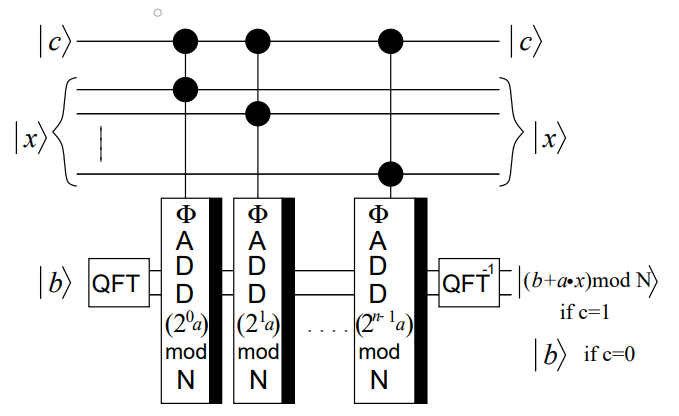
\includegraphics[scale = 0.6]{cmult.png}
  \caption{Kontrollierte Multiplikation nach Beauregard~\cite{beauregard2003circuit}}
  \label{fig:cmult}
\end{figure}


\bigskip

Der Code, der einen Quantenschaltkreis als Gatter gemäß dem Konzept in Abbildung~\ref{fig:cmult} generiert, 
ist in der Funktion \texttt{cmult\_gate}~\ref{code:ModularMultiplication} definiert.

Die Funktion erwartet sowohl \(a\) als auch \(N\) als Parameter, 
jeweils in der Form einer Liste, welche die Zahl in Binärdarstellung beschreibt.
Dabei repräsentiert der erste Index beider Listen das Least-Significant-Bit.
Damit die unterliegenden modularen Addition Gatter für die korrekte Anzahl an Qubits gebildet werden, 
müssen die Listen jeweils die Länge n + 1 haben, wenn \(N\) der Größenordnung \(2^n\) entspricht.
Das Most-Significant-Bit sollte in beiden Listen dementsprechend den Wert \(0\) haben.
Des Weiteren erwartet die Funktion den Parameter \textit{x\_bits\_amount}, der angibt, 
wie viele Qubits das Quantenregister \(\ket{x}_n\) umfasst 
und somit \(n\) entspricht. 

Um die Position der Qubits zu beschreiben, 
definiert die Funktion vier Wertebereiche.
\textit{c\_qbit} liegt an der ersten Stelle des kontrollierten Multiplikation Gatters und 
ist für das Kontrollqubit \(\ket{c}_1\) vorhergesehen.
Die darauffolgenden Qubits umfassen das \(\ket{x}_n\) Quantenregister und bestehen aus insgesamt \(n\) Qubits, 
deren Position in \textit{c\_qbit} definiert ist.
Die Position des \(\ket{b}_{n+1}\) Quantenregisters wird in \textit{b\_qbits} beschrieben.
Aufgrund der unterliegenden Gatter umfasst das \(\ket{b}_{n+1}\) Quantenregister ein zusätzliches Qubit, 
welches als Borrow-Bit dient.
Die Position des letzten Qubit \(\ket{0}_1\), 
wird mit \textit{cond\_qbit} definiert.
Dieses Qubit dient als Bedingungs-Qubit für die unterliegenden modularen Addition Gatter.

Im Code~\ref{code:ModularMultiplication} wird in Zeile 9. die Quanten-Fourier-Transformation auf 
das \(\ket{b}_{n+1}\) Quantenregister angewandt.
In Zeile 10 bis 13 folgen die Gatter zur modularen Addition.
Da \((b + a \cdot x) \bmod N\) äquivalent ist zu \((b + (a \cdot x)\bmod N) \bmod N\)~\cite{koepf_modular_2021}, 
wird einem Gatter der modularen Addition nicht der Parameter \(2^i\cdot a\) übergeben, 
sondern \((2^i\cdot a)\bmod N\).
Andernfalls wäre es notwendig, 
zusätzliche Qubits zu verwenden, um \(2^i\cdot a\) zu speichern.

Wie man in Zeile 13. sieht, teilen sich alle modularen Additions Gatter das selbe Bedingungs-Qubit \(\ket{0}_1\), 
welches sich auf der Position von \textit{cond\_qbit} befindet.
Genau aus diesem Grund, wird bei dem Gatter zur modularen Addition das Bedingungs-Qubit zurückgesetzt.

Abschließend wird noch die inverse Quanten-Fourier-Transformation auf das \(\ket{b}_{n+1}\) Quantenregister anwendet und 
der Quantenschaltkreis in ein Quantengatter umgeformt.

\begin{listing}[H]

\begin{minted}[linenos, fontsize=\customsize]{python}
def cmult_gate(x_bits_amount: int,a_bin: list[int],N_bin: list[int]) -> qiskit.circuit.gate:  
  a_dez = binToDez(a_bin)
  N_dez = binToDez(N_bin)
  c_qbit = [0]
  x_qbits =  list(range(1, x_bits_amount + 1))
  b_qbits = list(range(1+x_bits_amount, 1 + x_bits_amount + len(a_bin)))
  cond_qbit = [1 + x_bits_amount + len(a_bin)]
  cmult_gate = qiskit.QuantumCircuit(1 + x_bits_amount + len(a_bin) + 1)
  cmult_gate.append(QFT_Gate(len(b_qbits),inverse = False, MSB_first = False), b_qbits)
  for i in range(0, len(x_qbits)):
      a_i = ((2**(i)) *  a_dez) % N_dez
      a_i_bin = dezToBin(a_i, len(a_bin))
      cmult_gate.append(modular_adder_gate(a_i_bin, N_bin),c_qbit+[x_qbits[i]]+b_qbits+cond_qbit)
  cmult_gate.append(QFT_Gate(len(b_qbits),inverse = True, MSB_first = False), b_qbits)
  cmult_gate = cmult_gate.to_gate()
  cmult_gate.name = "cmult " + str(a_dez) + " Mod " + str(N_dez)
  return cmult_gate
  \end{minted}
  \caption{Kontrollierte Multiplikation in Qiskit}
  \label{code:ModularMultiplication}
\end{listing}

In Qiskit wird der durch den Code gebildete Quantenschaltkreis wie in Abbildung~\ref{fig:cmult_qiskit} dargestellt.
Die Abbildung repräsentiert den Quantenschaltkreis für \(a = 11;~N = 15\).

Die Visualisierung der Kontroll-Abzweigungen ist anders als in den vorherigen Abbildungen dargestellt.
Dies liegt daran, dass die Kontrollqubits bereits in den unterliegenden Gattern, 
also der modularen Addition, 
definiert wurden.
Es ist möglich, die Kontrollqubits bei der Definition der modularen Adder Gatter auszulassen und 
stattdessen erst bei der Anwendung im kontrollierten Multiplikation Gatter anzuwenden, 
indem die Qiskit Funktion \textit{control} verwendet wird.
Dadurch wird der Kontrolleffekt auf das gesamte Gatter zur modularen Addition angewendet, 
wodurch ein ineffizienterer Quantenschaltkreis entsteht, 
wie bereits im Abschnitt~\ref{sub:modulareAddition} zur modularen Addition erwähnt.

Es ist zu beachten, dass die Gatter zur modularen Addition in Abbildung~\ref{fig:cmult_qiskit} zwar über 
alle Qubits des \(\ket{x}_n\) Registers verlaufen, 
jedoch ausschließlich durch das Qubit kontrolliert werden, 
das im modularen Additions-Gatter den Index 1 trägt.

\begin{figure} [H]
  \centering
  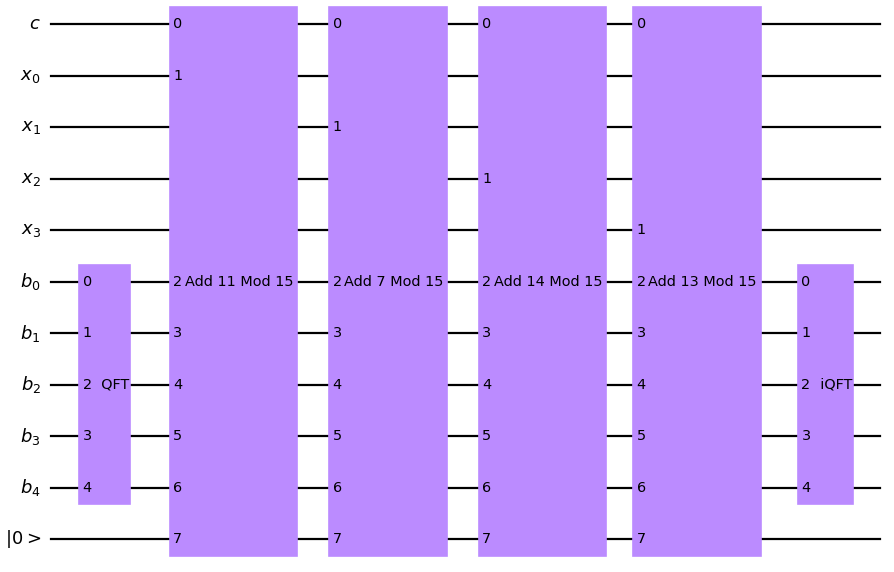
\includegraphics[scale = 0.5]{cmult_qiskit.PNG}
  \caption{Schaltkreis der kontrollierten Multiplikation in Qiskit}
  \label{fig:cmult_qiskit}
\end{figure}

Insgesamt wirkt das Gatter auf \(2n+3\) Qubits.
Diese setzen sich aus dem Kontrollqubit \(\ket{c}_1\), den \(n\) Qubits von \(\ket{x}_n\), 
den \(n+1\) Qubits von \(\ket{b}_{n+1}\) und dem einzelnen Bedingungs-Qubit \(\ket{0}_1\)zusammen.

Um der Inversen des kontrollierten Multiplikation Gatters eine eindeutige Benennung zu geben, 
wird dafür eine zusätzliche Funktion \texttt{inv\_cmult\_gate} definiert.
\begin{listing}[H]
\begin{minted}[linenos,fontsize=\customsize]{python}  
def inv_cmult_gate(x_bits_amount: int,a_bin: list[int],N_bin: list[int]) -> qiskit.circuit.gate:  
  inv_cmult_gate = cmult_gate(x_bits_amount,a_bin,N_bin).inverse()
  inv_cmult_gate.name = "inv cmult " + str(binToDez(a_bin)) + " Mod " + str(binToDez(N_bin))
  return inv_cmult_gate
  \end{minted}
  \caption{Inverse kontrollierte Multiplikation in Qiskit}
  \label{code:InverseModularMultiplication}
\end{listing}

\subsubsection{Vollständige Transformation}

Das letzte zu konstruierende Gatter wird als \(U_a\)-Gatter bezeichnet, 
weil es die benötigte Transformation realisiert: 
\[U^{\tensor n}\ket{y}_n = \ket{ay \bmod N}_n\] 
Das \(U_a\)-Gatter dient zur Realisierung der Quantum"=Phase"=Estimation im Shor"=Algorithmus, 
wie in Abbildung~\ref{fig:shor_n_qubit} dargestellt.

Dafür nimmt das \(U_a\)-Gatter vier Quantenregister entgegen und 
führt die folgende Transformation durch: 
\[\ket{c}_1\ket{x}_{n}\ket{0}_{n+1}\ket{0}_1
\longrightarrow
\ket{c}_1\ket{(a x) \bmod N}_{n}\ket{0}_{n+1}\ket{0}_1
\]

Um ein \(U_a\)-Gatter zu realisieren, benötigt man im Grunde kontrollierte Swap-Gatter und 
lediglich zwei Gatter zur kontrollierten Multiplikation. 
 
Im Folgenden wird die Auswirkung der einzelnen Bestandteile des \(U_a\)-Gatter erklärt.
Dabei werden von den vier Quantenregistern nur die beiden 
Quantenregister \(\ket{x}_{n}\ket{0}_{n+1}\) beachtet.
Das Qubit \(\ket{c}_1\) wie auch \(\ket{0}_1\) verzeichnet während der Transformation keine Veränderung, 
welche für das Verständnis des \(U_a\)-Gatter relevant ist.

Der Ablauf des \(U_a\)-Gatter lautet wie folgt:
Als erstes wird ein Gatter zur kontrollierten Multiplikation mit \(a\) angewendet. 
Dieses Gatter führt, 
ausgehend vom initialen Zustand der beiden Quantenregister, 
die folgende Transformation durch~\cite{beauregard2003circuit}:
\[
  \ket{x}_{n}\ket{0}_{n+1}
  \longrightarrow
  \ket{x}_{n}\ket{(ax)\bmod N}_{n+1}
  \]

Darauf folgen kontrollierte Swap-Gatter, die beide Zustände vertauschen:
\[
  \ket{x}_{n}\ket{(ax)\bmod N}_{n+1}
\longrightarrow
\ket{(ax)\bmod N}_{n}\ket{x}_{n+1}
\]
Dabei ist zu beachten, 
dass das zweite Quantenregister aus \(n+1\) Qubits besteht und
somit ein Qubit mehr besitzt als das erste Quantenregister.
Da das Most-Significant-Bit des zweiten Quantenregisters zu diesem Zeitpunkt garantiert im Zustand \(\ket{0}\) ist, 
kann es vernachlässigt werden und wird daher keiner Swap-Operation unterzogen.

Nach dem Swap wird ein inverses Gatter zur kontrollierten Multiplikation angewendet.
Dabei wird dem inversen Gatter zur kontrollierten Multiplikation statt dem Element \(a\) 
das multiplikative Inverse von \(a\) in den Einheiten des Restklassenrings \(N\) übergeben, 
also \(a^{-1} \bmod N\).
Als Folge davon verändert sich der Zustand der Quantenregister folgendermaßen:  
\[\ket{(ax)\bmod N}_{n}\ket{x}_{n+1}
\longrightarrow
\ket{(ax)\bmod N}_{n}\ket{(x-a^{-1}ax)\bmod N}_{n+1}
\] 
Der Ausdruck \((a^{-1}a)\bmod N\) entspricht dem neutralen Element 1, 
weswegen der Zustand der Quantenregister wie folgt vereinfacht werden kann:  
\[
\ket{(ax)\bmod N}_{n}\ket{(x-a^{-1}ax)\bmod N}_{n+1}
=
\ket{(ax)\bmod N}_{n}\ket{0}_{n+1}
\] 

Beachtet man den Eingangs- und Ausgangszustand der beiden Quantenregister, 
so bewirkt das \(U\)-Gatter eine Transformation von:
 \[\ket{x}_{n}\ket{0}_{n+1} 
 \longrightarrow 
 \ket{(ax)\bmod N}_{n}\ket{0}_{n+1}\]

Das Konzept des Aufbaus des Quantenschaltkreises ist in Abbildung~\ref{fig:u_gatter} dargestellt.
\begin{figure} [H]
  \centering
  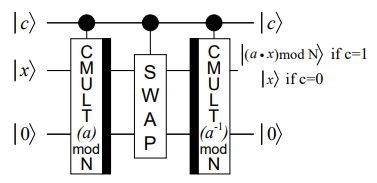
\includegraphics[scale = 0.8]{u_gatter.png}
  \caption{\(U_a\)-Gatter~\cite{beauregard2003circuit}}
  \label{fig:u_gatter}
\end{figure}

Die Funktion \texttt{U\_gate}~\ref{code:UGatter} enthält den Code zur Generierung eines \(U_a\)-Gatters.
Dazu nimmt die Funktion dieselben Parameter wie die Funktion \texttt{cmult\_gate} entgegen, 
nämlich  \textit{a\_bin} und \textit{N\_bin}, welche jeweils \(a\) und \(N\) in binärer Form im Listenformat beschreiben,  
sowie \textit{x\_bits\_amount}, das im Grunde \(n\) repräsentiert.

Im Code~\ref{code:UGatter} werden insgesamt fünf Wertebereiche definiert.
Das Kontrollqubit \(\ket{c}_1\) befindet sich auf der Position \textit{c\_qbit},
gefolgt von \textit{x\_qbits} für das \(\ket{x}_{n}\) Quantenregister und  
\textit{b\_qbits} für die Qubits von \(\ket{0}_{n+1}\).
Das Bedingungs-Qubit wird auf der letzten Position des Gatters platziert und  
ist in \textit{cond\_qbit} festgelegt.
Des Weiteren wird \textit{full\_range} verwendet,
um alle vier vorherigen Quantenregister zu umfassen.

Wie in Zeile 7. des Codes ersichtlich, wird zuerst ein Gatter zur kontrollierten Multiplikation eingesetzt.
Dafür werden der Funktion \texttt{cmult\_gate} die Parameter \textit{a\_bin}, \textit{N\_bin} und \textit{x\_bits\_amount} übergeben.
Das Gatter zur kontrollierten Multiplikation wird auf den gesamten Bereich \textit{full\_range} angewendet, 
somit umfasst das \(U_a\)-Gatter \(2n+3\) Qubits.
In Zeile 9 und 10 werden die kontrollierten Swap-Gatter eingesetzt.
Wie man in Zeile 10. erkennt, bezieht sich die Wirkung eines Swap-Gatters auf denselben Index von \textit{x\_qbits} und \textit{b\_qbits}.
Somit werden die Qubits beider Quantenregister vertauscht, die die gleiche Wertigkeit haben.
In Zeile 11. wird \(a^{-1}\bmod N\) mittels des erweiterten euklidischen Algorithmus berechnet.
Anschließend wird das berechnete \(a^{-1}\bmod N\) als Parameter an ein inverses kontrolliertes Multiplikation Gatter übergeben.
Abschließend wird der Quantenschaltkreis zu einem Gatter umgeformt und passend benannt.

\begin{listing}[H]
\begin{minted}[linenos,fontsize=\footnotesize]{python}  
def U_gate(x_bits_amount: int,a_bin: list[int],N_bin: list[int]) -> qiskit.circuit.gate:  
  c_qbit = [0]
  x_qbits =  list(range(1, x_bits_amount + 1))
  b_qbits = list(range(1+x_bits_amount, 1 + x_bits_amount + len(a_bin)))
  cond_qbit = [1 + x_bits_amount + len(a_bin)]
  full_range = c_qbit + x_qbits + b_qbits + cond_qbit
  U_a_gate = qiskit.QuantumCircuit(len(full_range))
  U_a_gate.append(cmult_gate(x_bits_amount,a_bin ,N_bin), full_range)
  for i in (range(x_bits_amount)):
      U_a_gate.cswap(c_qbit,x_qbits[i],b_qbits[i])
  a_inv_bin = dezToBin(\gcd(binToDez(a_bin),binToDez(N_bin)),len(a_bin))
  U_a_gate.append(inv_cmult_gate(x_bits_amount,a_inv_bin ,N_bin), full_range)
  U_a_gate = U_a_gate.to_gate()
  U_a_gate.name = "  U_" + str(binToDez(a_bin))
  return U_a_gate
  \end{minted}
  \caption{\(U\)-Gatter in Qiskit}
  \label{code:UGatter}
\end{listing}

Der Quantenschaltkreis, der durch den Code~\ref{code:UGatter} gebildet wird, 
wird in Qiskit wie in Abbildung~\ref{fig:u_gatter_qiskit} dargestellt. 
Die Abbildung zeigt ein Beispiel für \(a=7\) und \(N=15\).

\begin{figure}[H]
  \centering
  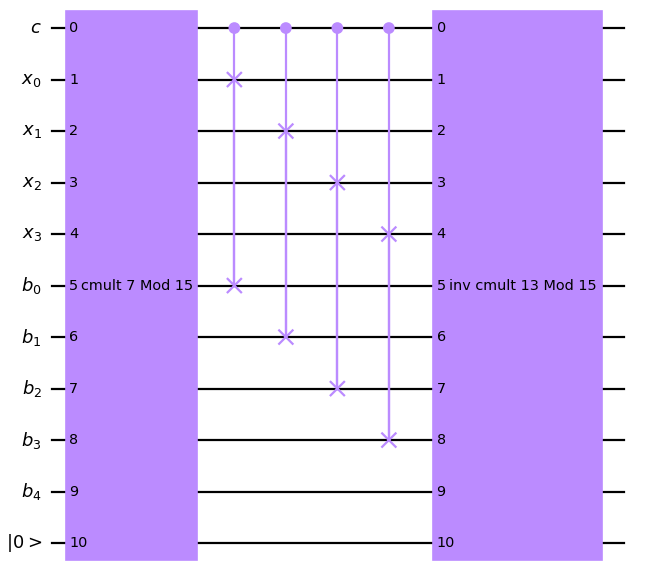
\includegraphics[scale = 0.5]{u_gatter_qiskit.PNG}
  \caption{\(U_a\)-Gatter in Qiskit}
  \label{fig:u_gatter_qiskit}
\end{figure}

\subsubsection{Quantum-Phase-Estimation für Shor} \label{section:imp_QPE_Shor}
Der letzte Schritt zur Komplettierung des Quantenschaltkreises für den Quantenalgorithmus, 
der in der Lage ist, 
die Periode zu bestimmen, besteht darin, 
die Quantum-Phase-Estimation wie in Abbildung~\ref{fig:shor_n_qubit} unter Verwendung des \(U_a\)-Gatters zu bilden.

In Abbildung~\ref{fig:shor_n_qubit} werden unter anderem \({U_a}^{2^x}\)-Gatter eingesetzt.
Diese können realisiert werden, 
indem ein \({U_a}\)-Gatter insgesamt \(2^x\) mal hintereinander geschaltet wird oder 
indem anstelle von \(a\) der Parameter \(a^{2^x}\) an ein einzelnes \(U_a\)-Gatter übergeben wird.
Die zweite Variante ist möglich wegen~\cite{beauregard2003circuit}:
\[(a^nx)\bmod N = \underbrace{(a\dotsc(((a(ax)\bmod N)\bmod N)\dotsc)\bmod N)}_{\text{\(n\) mal}}\]

Bei der Wahl zwischen den beiden Varianten liegt das entscheidende Kriterium bei der Ressourceneffizienz. 
Die zweite Variante schneidet dabei deutlich besser ab, 
da sie lediglich \(x\) viele \(U_a\)-Gatter benötigt, 
wenn \(x\) viele Kontrollqubits verwendet werden, 
im Gegensatz zur ersten Variante, die \(2^x-1\) viele \(U_a\)-Gatter erfordert.

Ein weiterer wichtiger Aspekt für den Aufbau der Quantenschaltung betrifft die Anzahl der benötigten Kontrollqubits.
Beauregard erklärt in seinem Paper~\cite{beauregard2003circuit} nicht, 
warum er eine Konstruktion mit insgesamt \(2n\) Kontrollqubits beziehungsweise \({U_a}^{2^x}\)-Gatter wählt.
Es gibt Quellen, die mehr als \(2n\)  Kontrollqubits verwendeten~\cite[229]{nielsen_chuang_2010}.
Nach dem Paper von Peter Shor~\cite{Shor_1997} sind jedoch \(2n\) Kontrollqubits ausreichend,
wie auch im Abschnitt~\ref{Funktionsweise:klassisch} erläutert wird.
Deswegen verwendet die hier implementierte Variante \(2n\) Kontrollqubits.

\bigskip

Der Code für einen Quantenschaltkreis wie in Abbildung~\ref{fig:shor_n_qubit} ist in der Funktion 
\texttt{Shor}~\ref{code:Periodenbestimmung} enthalten.

Die Funktion erwartet die beiden Zahlen \(a\) und \(N\) als Parameter.
Des Weiteren kann der Funktion über den Parameter \textit{number\_shots} mitgeteilt werden, 
mit wie vielen Durchläufen der Quantenalgorithmus ausgeführt werden soll.
Jeder Durchlauf gewährt ein weiteres Messergebnis.
Der Parameter \textit{backend} ist dazu da, 
um festzulegen, auf welchem System der Quantenalgorithmus ausgeführt werden soll.
Standardmäßig wird der Simulator von Qiskit genutzt. 
Falls Zugang zu einem Quantensystem von IBM besteht, 
würde man stattdessen die Bezeichnung der entsprechenden Quantum-Backend verwenden.

Die Funktion \texttt{Shor} definiert die beiden Wertebereiche \textit{c\_qbits} und 
\textit{ev\_qbits}, um die Positionen der beiden Quantenregister zu beschreiben.
Der Wertebereich \textit{c\_qbits} enthält die insgesamt \(2n\) Positionen der Kontrollqubits.
Der Eigenvektor wird in den Qubits gespeichert, 
deren Position in \textit{ev\_qbits} definiert ist.

Der Quantenschaltkreis wird in der 5. Zeile definiert und umfasst \(4n+2\) Qubits und 
\(2n\) klassische Bits, welche zum Messen verwendet werden.
In Zeilen 6 und 7 wird ein Hadamard-Gatter auf jedes Kontrollqubit angewendet.
In den der 8. Zeile wird der Eigenvektor gebildet. 
Da der Eigenvektor dem Zustand \(\ket{1}\) entspricht,
genügt es, wenn das Least-Significant-Qubit mit einem X-Gatter versehen wird.
In den Zeilen 9 und 10 werden die zugehörigen \({U_a}^{2^x}\)-Gatter mit dem passenden \(x\) auf das Register mit dem Eigenvektor angewendet.
Die Funktion \texttt{mod\_exp} berechnet \((a^{2^x})\bmod N\).
In der 11. Zeile werden die Kontrollqubits mit der inverse Quanten-Fourier-Transformation in die Standardbasis transformiert.  
Da die Funktion \texttt{Shor} Messungen durchführen soll, 
wird in der 12. Zeile definiert, dass die Kontrollqubits gemessen werden.
In dem Fall entspricht dies den Qubits auf den Positionen \textit{c\_qbits}.
Anschließend werden in den Zeilen 13 und 14 \textit{number\_shots} viele Messungen durchgeführt und 
das Ergebnis wird als Rückgabewert der Funktion zurückgegeben.

Wie bei der Definition des Quantenschaltkreises in Zeile 5. erkennbar, 
benötigt der Quantenschaltkreis \(4n+2\) Qubits anstatt \(2n+3\).
Die Reduktion der benötigten Qubits wird in der Sektion~\ref{Optimierung} thematisiert. 

\begin{listing}[H]
\begin{minted}[linenos,fontsize=\customsizetwo]{python}  
def Shor(a: int, N: int,number_shots: int = 1000, backend: str = "aer_simulator"):
  n = N.bit_length()
  c_qbits = range(2*n)
  ev_qbits = list(range(len(c_qbits),4*n+2))
  qc = qiskit.QuantumCircuit(4*n+2,len(c_qbits)) 
  for c_bit in c_qbits:
    qc.h(c_bit)
  qc.x(ev_qbits[0])
  for c_bit in c_qbits:
    qc.append(U_gate(n,dezToBin(mod_exp(a,2**c_bit,N),n+1),dezToBin(N,n+1)),[c_bit]+ev_qbits)
  qc.append(QFT_Gate(len(c_qbits),inverse = True, MSB_first = False,swaps = True), c_qbits)
  qc.measure(c_qbits,c_qbits)
  simulator = qiskit.Aer.get_backend(backend)
  sim_result = qiskit.execute(qc, backend=simulator, shots=number_shots).result()
  return sim_result.get_counts(qc)
  \end{minted}
  \caption{Periodenbestimmung in Qiskit}
  \label{code:Periodenbestimmung}
\end{listing}

In Abbildung~\ref{fig:shor_qiskit} ist der Quantenschaltkreis zu sehen, 
der durch die Funktion \texttt{Shor} für \(a=7;~N=15\) generiert wird.
Bei \(N=15\) tritt der Effekt auf, dass für \(x>1\) die Rechnung \((a^{2^x})\bmod N = 1\) ergibt, 
weshalb auch die \({U_a}^{2^x}\)-Gatter zu \(U\_1\) werden.

\begin{figure}[H]
  \centering
  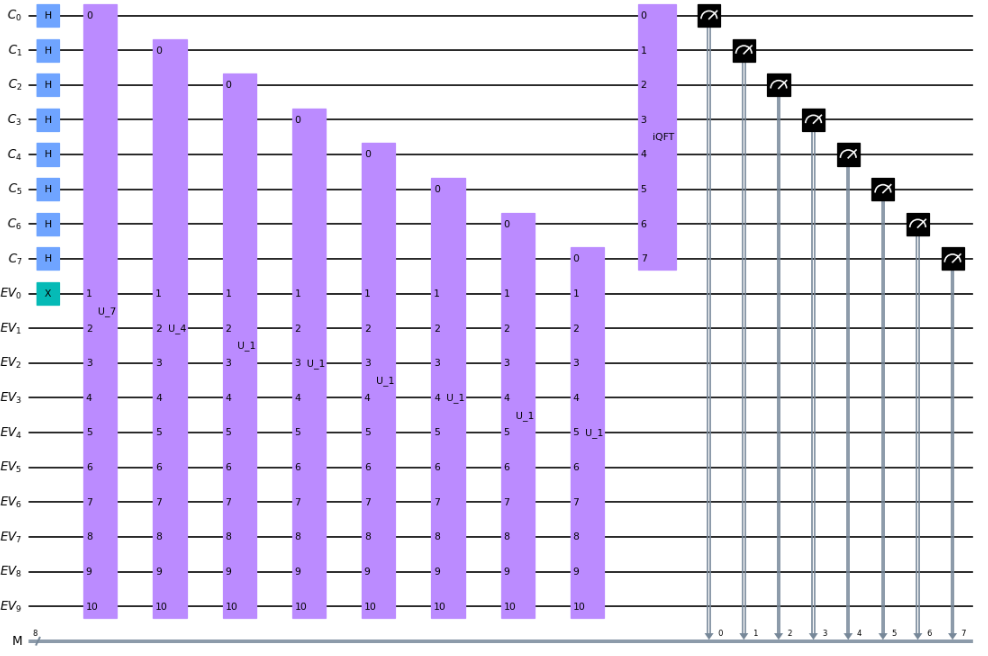
\includegraphics[scale = 0.6]{shor_qiskit.PNG}
  \caption{Quantenalgorithmus von Shor in Qiskit}
  \label{fig:shor_qiskit}
\end{figure}

\subsection{Faktorisierungsalgorithmus} \label{sec:Faktorisierungsalgorithmus}
Der Faktorisierungsalgorithmus kombiniert die Quantum-Phase-Estimation zur Periodenberechnung mit  
der klassischen Nachberechnung. 
Der Hauptfokus der Implementierung liegt darauf, 
die Schwächen der Messergebnisse der Quantum-Phase-Estimation mithilfe klassischer Methoden zu kompensieren.

Es ist zu erwarten, 
dass die Ausführung von Quantenberechnungen auch mit zukünftig fortschrittlichen Quantencomputern kostenintensiv sein wird~\cite{Shor_1997}.
Daher wäre es ineffizient, 
die Quantum-Phase-Estimation so oft zu wiederholen, 
bis ein Ergebnis erzielt wird, dass die Periode direkt offenbart.
Stattdessen ist es ressourcensparender, 
ein erhaltenes Messergebnis, 
unter Berücksichtigung der in Abschnitt~\ref{Funktionsweise:klassisch} erklärten drei möglichen Szenarien,
mit klassischen Methoden aufzubereiten. 
Als Resultat können so weitere Durchläufe der Quantum-Phase-Estimation eingespart und 
durch klassische Rechenleistung ersetzt werden.

\bigskip

Die Grafik~\ref{fig:shor_measure} repräsentiert insgesamt 512 Messungen für \(a=19;~N=119\), 
mit einer Genauigkeit \(k\) von \(2\ld(119) \approx 14 \). 
Ihr Zweck ist es, die Besonderheiten, 
welche bei Messergebnissen auftreten können, hervorzuheben.
Zur Verdeutlichung sind die Messergebnisse in Abbildung~\ref{fig:shor_measure} in vier Kategorien eingeteilt.
Die Kriterien für die Einteilung in diese Kategorien basieren darauf, 
ob nach der Division durch \(2^k\) und 
der Anwendung des Kettenbruch-Algorithmus mit einem Nenner kleiner als \(N\), 
die Periode erfolgreich extrahiert werden kann.

Die grünen Ergebnisse offenbaren direkt die gesuchte Periode von \(p = 24\).
Ein Faktorisierungsalgorithmus, welcher so lange die Quantum-Phase-Estimation wiederholt, 
bis ein Messergebnis die ungekürzte Periode enthält, 
wird ausschließlich bei den grünen Ergebnissen erfolgreich sein.

Anhand der gelben Ergebnisse kann die gesuchte Periode nicht direkt extrahiert werden.
Dabei ist der Fall eingetreten, dass der Zähler und Nenner des Bruches einen gemeinsamen Teiler hatten, 
weshalb der Bruch gekürzt wurde.
Gegebenenfalls kann die Periode mit klassisch ausführbaren Methoden rekonstruiert werden.

Die hellroten Ergebnisse sind zu weit vom Peak entfernt,
weswegen diese die gesuchte Periode weder vollständig noch gekürzt enthalten.
Womöglich kann die Periode aus diesem Messergebnis ermittelt werden, 
wenn die benachbarten Zustände überprüft werden.

Die beiden dunkelroten Zustände sind die beiden Zustände der finalen Superposition
\(\ket{2^k \cdot \frac{0}{p}}_k\) und \(\ket{2^k \cdot \frac{p/2}{p}}_k\).
Der Zustand \(\ket{2^k \cdot \frac{0}{p}}_k\) existiert für jede Zahl und erlaubt keine 
Rückschlüsse auf die Periode.
Der andere Zustand \(\ket{2^k \cdot \frac{p/2}{p}}_k\) existiert ausschließlich, wenn \(p\) gerade ist.
Auch dieser Zustand gewährt keine hilfreichen Rückschlüsse auf die Phase, 
da \(\frac{p/2}{p}\) immer zu \(\frac{1}{2}\) gekürzt wird.
Eine notwendige Bedingung, um die Faktoren aus \(p\) herleiten zu können, 
ist, dass \(p\) gerade ist~\cite*{Shor_1997}, 
dies wird zwar durch die Messung von \(\ket{2^k \cdot \frac{p/2}{p}}_k\) bestätigt, 
jedoch kann aus dieser Information keine hilfreiche Konsequenz gezogen werden.

\begin{figure}[H]
  \centering
  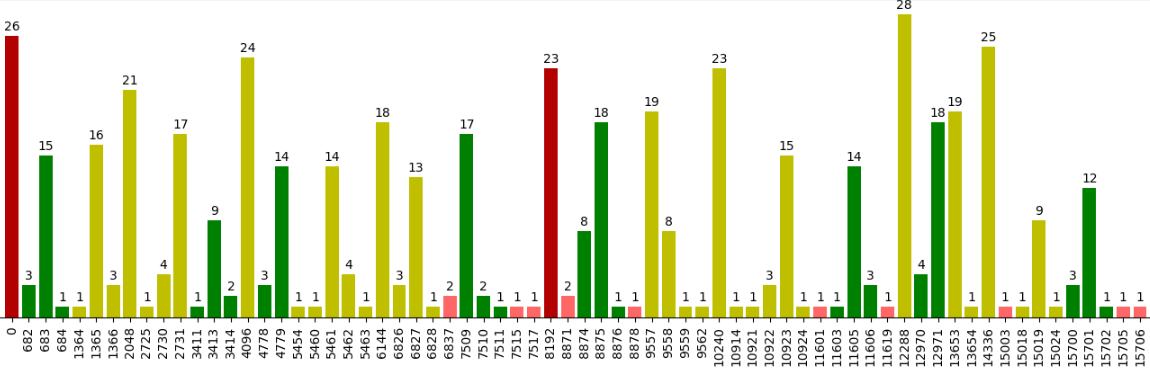
\includegraphics[scale = 0.5]{Messung_beispiel.PNG}
  \caption{Beispiel Messung a=19, N=119, k=14}
  \label{fig:shor_measure}
\end{figure}


\bigskip

Abbildung~\ref{fig:Flussdiagramm} gibt einen Überblick über den Ablauf des Algorithmus 
von der Berechnung der Periode bis zur Bestimmung der Primfaktoren.

Am Anfang des Algorithmus wird zufällig ein \(a\) definiert, 
welches größer als 1, aber kleiner als \(N\) ist.

Für den ungewöhnlichen Fall, dass \(a\) einen gemeinsamen, nicht-trivialen Teiler mit \(N\) hat, 
ist dieser einer der gesuchten Faktoren von \(N\), 
weswegen der Algorithmus terminiert.
Die Überprüfung, ob \(a\) und \(N\) einen Faktor teilen, 
kann mit Euklids Algorithmus mit maximal polynomialen Aufwand berechnet werden~\cite[301]{homeister2023quantum215}. 
Euklids Algorithmus ist in der Lage, den größten gemeinsamen Teiler (\(\gcd\)) zu berechnen.

Anschließend wird zu dem gewählten \(a\) ein Set erstellt.
Dieses Set wird dafür genutzt, um die Brüche zu speichern, 
bei denen die Periode nicht im Nenner steht. 
Die gespeicherten Brüche enthalten in ihrem Nenner womöglich Teiler der gesuchten Periode, 
welche bei weiteren Berechnungen dabei helfen könnten, die Periode zu finden.

Darauf folgt der einzige quantenalgorithmische Bestandteil der Berechnung, 
welcher auf einem Quantencomputer ausgeführt wird.
Konkret geht es um die Ausführung der für die Periodenbestimmung angepassten Quantum-Phase-Estimation. 
Für ein ressourceneffizienteres Vorgehen wird nur ein Durchlauf der Quantum-Phase-Estimation angestoßen.
Anhand des einzelnen Messergebnisses wird die Berechnung fortgesetzt.

Die nächsten Berechnungen werden wieder auf einem klassischen Rechnersystem ausgeführt.
Bei der Berechnung wird das Messergebnis aus dem Binärsystem ins Dezimalsystem umgewandelt
und durch die entsprechende 2er-Potenz geteilt.
Nachdem das Ergebnis ermittelt wurde, 
wird der Kettenbruch-Algorithmus angewendet. 
Dieser Algorithmus findet aufgrund der festgelegten Limitation den nächstgelegenen Bruch mit einem Nenner kleiner als \(N\).
Dieser Schritt ist ebenfalls mit einem maximal polynomialen Aufwand durchführbar~\autocite[230]{nielsen_chuang_2010}.

Im nächsten Schritt wird überprüft, ob der Nenner des Bruches der Periode entspricht.
Im ersten Durchlauf wird dies nur der Fall sein, 
wenn die Messung einen der Zustände ergeben hat, 
die wie in Abbildung~\ref{fig:shor_measure} zu der farblich grünen Kategorie gehört.
Sollte es nicht möglich sein, die Periode direkt zu extrahieren, 
wird anhand des Messergebnisses eine Nachberechnung angestoßen.

Der erste Schritt in der Nachberechnung besteht darin, 
zu überprüfen, ob ein Vielfaches des Nenners die Periode darstellt.
Dabei ist zu beachten, bis zu welchem Vielfachen diese Überprüfung durchgeführt wird. 
Ein sinnvoller Ansatz wäre, eine Obergrenze festzulegen, die logarithmisch mit \(n\) wächst.
Andernfalls könnte es bei sehr großen Werten für \(N\) passieren, 
dass zu viele klassische Berechnungen anfallen würden, die in keinem vertretbaren Zeitaufwand durchführbar wären.
In der Implementierung werden die Vielfachen mit einer Multiplikation von \(2\) bis \(2^{\ld(n)}\) getestet.

Sollte die Periode keines der getesteten Vielfachen des Nenners darstellen, 
wird das kleinste gemeinsame Vielfache(kgV) des aktuellen Nenners mit den einzelnen Nennern aus dem Set gebildet.
Falls die beiden zugehörigen Zähler keinen Faktor teilen, 
kann mit einer Wahrscheinlichkeit größer als \(0.25\) die Periode aus dem kgV berechnet werden~\cite[231]{nielsen_chuang_2010}.

Die beiden vorherigen Methoden können zum Erfolg führen, 
falls ein Messergebnis, wie in Abbildung~\ref{fig:shor_measure}, 
zur gelben Kategorie gehört. 

Wenn beide vorherigen Methoden fehlschlagen, 
wird angenommen, dass das Messergebnis einer der beiden roten Kategorien angehört.
In diesem Fall wird überprüft, ob einer der Nachbarn die Periode enthält.
Damit der Aufwand nicht den Rahmen der Laufzeit sprengt, 
werden genau wie bei der Überprüfung der Vielfachen
nur eine begrenzte Anzahl an Nachbarn getestet.
Genau wie bei der Überprüfung der Vielfachen werden in der Implementierung alle Nachbarn durch 
die Addition beziehungsweise Subtraktion des Messwertes von \(1\) bis \(2^{\ld(n)}\) getestet.

Falls einer der Nachbarn die Periode enthält, 
handelt es sich bei dem Zustand des Nachbarn um einen, 
welcher der grünen Kategorie angehört, 
wie beispielsweise in Abbildung~\ref{fig:shor_measure} der Zustand \(\ket{8878}_{14}\).

Es ist möglich, 
dass die Zustände der Nachbarn des Messergebnisses der gelben Kategorie angehören.
In diesem Fall ist eine direkte Extraktion nicht möglich, 
weswegen auch die Vielfachen und das kgV von einem benachbarten Zustand geprüft wird.
In Abbildung~\ref{fig:shor_measure} repräsentiert der Zustand \(\ket{6837}_{14}\) dieses Szenario.

Sollte trotz der Nachberechnung keine Periode extrahiert werden können, 
wird der Bruch des Messergebnisses im Set gespeichert.
Anschließend wird ein neuer Durchlauf der Quantum-Phase-Estimation 
mit demselben \(a\) durchgeführt.

Im Falle, dass die Periode direkt extrahiert werden konnte oder 
durch die Nachberechnung bestimmt wurde, wird überprüft, 
ob die Periode einer geraden Zahl entspricht und die folgende Bedingung erfüllt:
\[a^{\frac{p}{2}} = -1 \bmod N\]
Wenn beide Kriterien zutreffen, 
kann mit der Periode und 
Euklids Algorithmus mindestens einer der beiden nicht-trivialen Faktoren von \(N\) berechnet werden~\cite{Shor_1997}:
\[\gcd(a^{\frac{p}{2}}-1, N), \gcd(a^{\frac{p}{2}}+1, N)\]
Anschließend terminiert der Algorithmus. 

Im Falle, dass nur ein Faktor gefunden wurde, kann der zweite berechnet werden, 
indem \(N\) durch den gefundenen Faktor dividiert wird.

Falls die Periode ungerade ist oder die zweite Bedingung nicht erfüllt ist, 
ist es nicht möglich, aus der gefundenen Periode die Faktoren zu berechnen~\cite{Shor_1997}.
In diesem Fall wird ein neues \(a\) gewählt und ein neues leeres Set definiert. 
Das alte Set beinhaltet Informationen zur Periode des vorherigen \(a\).
Anschließend wird mit dem neuen \(a\) die Quantum-Phase-Estimation ausgeführt und 
die Berechnung wiederholt.

Im Flussdiagramm und in der Beschreibung 
wird die Ausführung des Quantenalgorithmus praktisch als ein sequenzieller Abschnitt dargestellt, 
welcher erst durch einen gewissen Punkt in der klassischen Berechnung angestoßen wird.
Dies ist aber nur der Fall, bis das erste \(a\) bestimmt wird.
Da der Quantenalgorithmus und die klassischen Berechnungen auf zwei unterschiedlichen Systemen laufen~\cite{IBMQuantumServerless2023}, 
ist es möglich, parallel zur klassischen Nachberechnung, 
bereits einen weiteren Durchlauf der Quantenberechnung durchzuführen. 
Allerdings kann es bei diesem Vorgehen dazu kommen, 
dass die erste Messung bereits die korrekte Periode offenbart, 
weswegen eine parallele zweite Messung unnötige Quanten-Ressourcen beansprucht.

\begin{figure} 
  \centering
  % Use textheight minus 1 line for caption minus 1 line skip
  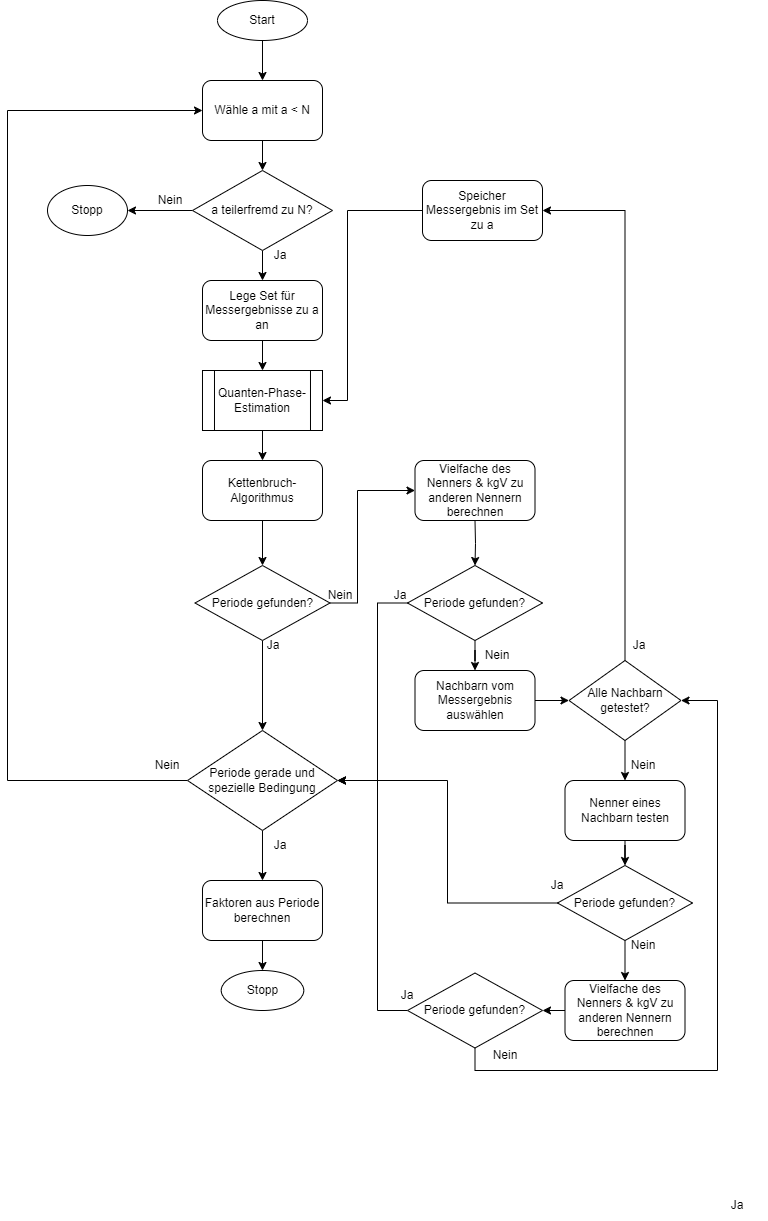
\includegraphics[height=\dimexpr\textheight-2\baselineskip]{FlussdiagramFaktorisierung.png}
  \caption{Flussdiagramm Faktorisierung}
  \label{fig:Flussdiagramm}
\end{figure}

\subsection{Optimierung} \label{Optimierung}
Die folgende Sektion thematisiert zwei mögliche Methoden, 
um den Ressourcenbedarf der Quantenbrechung zu reduzieren.
Beide Optimierungen kommen mit einer Abwägung, 
die gewisse Nachteile mit sich bringt,
wodurch im Gegenzug jedoch Ressourcen eingespart werden.
Somit handelt es sich bei den Optimierungen um Lösungen, 
die situationsbedingt besser sind.
Dabei sind die Eigenschaften und die Architektur des genutzten Quantencomputers die ausschlaggebenden Kriterien.

\subsubsection{Iterative Quantumten-Phase-Estimation}
In den vorherigen Kapiteln wurde die Quantum-Phase-Estimation in der Standardvariante, 
wie in Sektion~\ref{Quanten-Phase-Estimation} beschrieben, verwendet.
In der Standardvariante wird für jedes \(U^{2^x}\)-Gatter ein eigenes Kontrollqubit benötigt.
Dies bedeutet, wenn \(2n\) viele \(U^{2^x}\)-Gatter angewendet werden sollen, 
sind genau so viele Kontrollqubits nötig.

Ein zentraler Bestandteil der Quantum-Phase-Estimation ist die (inverse) Quanten-Fourier-Transformation. 
Wie im Abschnitt~\ref{Quanten-Fourier-Transformation} gezeigt, 
hängt die Wirkung dieser Transformation auf ein einzelnes Qubit von den Zuständen der anderen Qubits ab 
und zwar aufgrund von kontrollierten Phasenverschiebungen.

Bei der regulären Quanten-Fourier-Transformation kontrolliert ein bestimmtes Qubit zunächst die Phasen-Gatter auf die übrigen Qubits, 
bevor auf das kontrollierende Qubit selbst ein Hadamard-Gatter angewendet wird.
Das bedeutet, dass die kontrollierten Gatter der regulären Quanten-Fourier-Transformation abhängig sind von dem Eingangszustand.

Dies sieht bei der inversen Quanten-Fourier-Transformation anders aus.
Bei der inversen Quanten-Fourier-Transformation wird auf ein Qubit zuerst ein Hadamard-Gatter angewendet, 
erst danach kontrolliert es die Phasen-Gatter auf die anderen Qubits.
Dementsprechend sind bei der inversen Quanten-Fourier-Transformation die kontrollierten Gatter abhängig von dem Ausgangszustand.

Die Abhängigkeit zum Ausgangszustand ermöglicht es, 
die inverse Quanten-Fourier-Transformation aufzuteilen und die Bestandteile iterativ anzuwenden.
Dadurch wird der Ressourcenbedarf der Quantum-Phase-Estimation von \(2n\) Kontrollqubits auf ein einzelnes reduziert~\cite{Parker2000}.

In der Standardvariante der Quanten-Fourier-Transformation kontrollieren Qubits die Phasen-Gatter.
In der semi-klassischen beziehungsweise, iterativen Variante ist dies anders.
Diese Methode kam erstmals 1995 zum Einsatz und 
nutzt das klassische Signal einer Messung, 
um ein Quanten-Gatter zu kontrollieren~\cite{Griffiths_1996}.
Im Kern der Optimierung liegt der Trick darin, 
das Messergebnis des jeweiligen Qubits als Steuerungsbedingung für ein Phasen-Gatter zu verwenden.

Die Quantum-Phase-Estimation verwendet die inverse Quanten-Fourier-Transformation mit Swap-Gattern.
Da die identische Transformation benötigt wird, 
muss die iterative Variante das Verhalten der Swap-Gatter berücksichtigen.
Zur besseren Verständlichkeit ist die inverse Quanten-Fourier-Transformation mit Swap-Gattern in Abbildung~\ref{fig:iQFTswaps} dargestellt.
\begin{figure}[H]
  \centering
  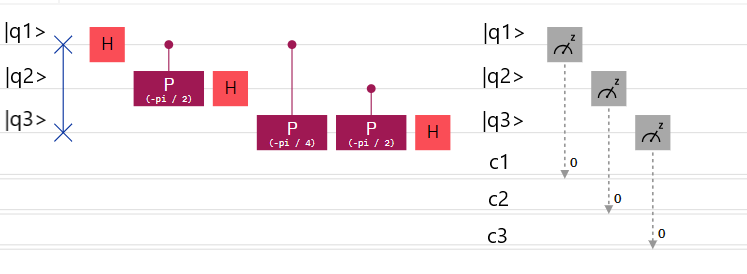
\includegraphics[scale = 0.6]{iqft_3qubit_swaps.PNG}
  \caption{3 Qubits inverse QFT mit Swaps}
  \label{fig:iQFTswaps}
\end{figure}
Wie in Abbildung~\ref{fig:iQFTswaps} dargestellt, 
wird das Eingangsqubit \(\ket{q3}_1\), welches das Most-significant-Bit enthält, 
mit \(\ket{q1}_1\) getauscht. 
Anschließend wird ein Hadamard-Gatter angewendet, 
wodurch das \(\ket{q3}_1\) Qubit in die Standardbasis transformiert wird. 
Erst danach kontrolliert das \(\ket{q3}_1\) Qubit zwei Phasen-Gatter.
Der Messwert wird in dem klassischen Bit \(c1\) gespeichert.
Das gleiche Verhalten kann, wie in Abbildung~\ref{fig:iterative_iQFT} gezeigt, nachgestellt werden, 
indem nach der Anwendung des Hadamard-Gatters auf das \(\ket{q3}_1\) Qubit 
der Messwert im klassischen Bit \(c1\) gespeichert wird.
Anschließend kontrolliert das klassische Bit \(c1\) die Phasen-Gatter.

Um nach der Messung dasselbe Kontrollqubit für \(\ket{q2}_1\) verwenden zu können, 
muss dieses in einen eindeutigen Zustand versetzt werden, 
in diesem Fall der Zustand \(\ket{0}\).
Aufgrund der zuvor durchgeführten Messung 
kollabiert der Zustand des Qubit zu \(\ket{0}\) oder \(\ket{1}\). 
Wenn der Zustand der \(\ket{1}\) entspricht, 
wird ein X-Gatter kontrolliert angewendet, 
welches durch das Messergebnis aus \(c1\) kontrolliert wird. 
Somit befindet sich das Qubit in beiden Fällen im Zustand \(\ket{0}\).

Anschließend beginnt die Sequenz für das \(\ket{q2}_1\) Qubit.
Das bedeutet, dass alle Operationen, die von dem \(\ket{q2}_1\) Qubit abhängig sind, 
jetzt erst angewendet werden.
Im Kontext der Quantum-Phase-Estimation wird an dieser Stelle das zugehörige \(U^{2^x}\)-Gatter von \(\ket{q2}_1\) kontrolliert.
In Abbildung~\ref{fig:iterative_iQFT} entspricht dies der Stelle, an der die Bezeichnung \(\ket{q2}\) steht.
Im nächsten Schritt werden die Gatter der Quanten-Fourier-Transformation angewendet, gefolgt von einer Messung. 
Das Ergebnis dieser Messung wird in einem weiteren klassischen Bit gespeichert, in diesem Fall \(c2\).
Für \(\ket{q1}_1\) ist der Ablauf fast identisch.
Der einzige Unterschied besteht darin, 
dass nun zwei kontrollierte Phasen-Gatter angewendet werden, 
von denen eines von \(c1\) und das andere von \(c2\) kontrolliert wird.
Abschließend wird das Messergebnis von \(\ket{q1}_1\) in einem weiteren klassischen Bit \(c3\) gespeichert.

Die verdrehte Reihenfolge beim Speichern der Messergebnisse dient dazu, 
den Effekt der Swap-Gatter nachzubilden.
\begin{figure}[H]
  \centering
  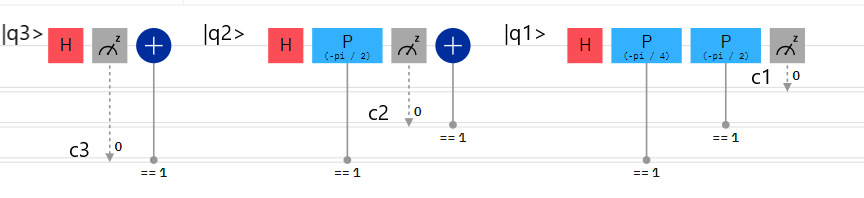
\includegraphics[scale = 0.6]{iterative_iqft.PNG}
  \caption{3 Messungen inverse iterative QFT}
  \label{fig:iterative_iQFT}
\end{figure}
  
Wie im vorherigen Absatz erwähnt, 
werden bei der iterativen Quantum"=Phase"=Estimation die \(U^{2^x}\)-Gatter zwischen den Abschnitten 
der iterativen Quanten"=Fourier"=Transformation angewendet. 

Als Ergebnis besitzt der Quantenschaltkreis für den Shor Algorithmus mit der iterativen Quantum-Phase-Estimation eine grundlegend andere Struktur 
im Vergleich zur regulären Variante.
Dies resultiert darin, dass die iterative Quanten-Fourier-Transformation kein zusammenhängender Baustein ist, 
sondern dass die einzelnen Bestandteile schrittweise zwischen 
den einzelnen \(U^{2^x}\)-Gatter angewendet werden.

\bigskip

Aufgrund der benötigten klassisch-kontrollierten Phasen-Gatter wird die iterative Quanten-Fourier-Transformation nicht als einzelne Gatter, 
sondern in einer Funktion \texttt{iterative\_QFT} definiert.
Diese Funktion wendet die erforderlichen klassisch-kontrollierten Gatter direkt auf den Quantenschaltkreis für ein jeweiliges Qubit an.

Wie im Code in Abbildung~\ref{code:iterativeQFT} dargestellt, 
erwartet die Funktion \texttt{iterative\_QFT} die vier Parameter: \textit{target}, \textit{qc}, \textit{k} und \textit{controlling\_qubit}.
Der Parameter \textit{target} beschreibt die Wertigkeit des Qubits und 
definiert zusammen mit der Genauigkeit \textit{k}, 
welche Phasen-Gatter benötigt werden.
Alle durch die Funktion \texttt{iterative\_QFT} angewendeten Gatter 
werden auf den Quantenschaltkreis im Parameter \textit{qc} angewendet.
Der letzte Parameter, \textit{controlling\_qubit}, beinhaltet das Ziel der angewendeten Gatter und 
somit die Position des Kontrollqubit.

Wenn der Parameter \textit{target} dem Wert 0 entspricht, 
wird die iterative Quanten-Fourier-Transformation für das Most-Significant-Bit angewendet.
Wie in Abbildung~\ref{fig:iterative_iQFT} gezeigt, entspricht dies nur der Anwendung eines einzelnen Hadamard-Gatters.
In Zeile 3 und 4 ist zu erkennen, 
dass mit abnehmender Wertigkeit eines Qubits zunehmend mehr Phasen-Gatter angewendet werden.
Alle Phasen-Gatter, welche in Zeile 4. genutzt werden, 
wirken auf das \textit{controlling\_qubit} und 
werden von unterschiedlichen klassischen Bits mit der Methode \(c\_if\) kontrolliert.

Da die Funktion direkt auf den Quantenschaltkreis \textit{qc} wirkt, 
wird kein Rückgabewert benötigt.
\begin{listing}[H]
\begin{minted}[linenos,fontsize=\footnotesize]{python}    
def iterative_QFT(target: int, qc: QuantumCircuit ,k: range, controlling_qubit: int):
    if target != 0:
        for i in list(reversed(range(target))):
            qc.p((-pi/(2**(i+1))),controlling_qubit).c_if(k[target - (i+1)],1)
    qc.h(controlling_qubit)
  \end{minted}
  \caption{Part Iterative QFT in Qiskit}
  \label{code:iterativeQFT}
\end{listing}

Der Code zum vollständigen Quantenschaltkreis ist in Abbildung~\ref{code:IterativeQPE} in der Funktion \texttt{Shor\_sequential} dargestellt.
Die Parameter sind identisch mit denen der regulären \texttt{Shor} Funktion. 
Wie in Zeile 6. der Quantenschaltkreis-Definition zu erkennen ist, 
benötigt diese Variante insgesamt \(2n+3\) Qubits und halbiert damit fast den Bedarf der Standardvariante von \(4n+2\) Qubits.
In den Zeilen 8 bis 14 ist ersichtlich, 
dass die Komponenten der iterativen Quanten-Fourier-Transformation in jedem Schleifendurchlauf nach einem \(U^{2^x}\)-Gatter angewendet werden. 
Des Weiteren ist ersichtlich, 
dass die Schleife mit dem Qubit beginnt, 
welches die höchste Wertigkeit (Most-Significant-Bit) hat.
Pro Iteration wird jeweils ein \(U^{2^x}\)-Gatter mit absteigender Potenzen zum vorherigen Durchlauf angewendet, 
hingegen werden die Messergebnisse in klassischen Bits mit aufsteigender Wertigkeit gespeichert.

Um zu verhindern, 
dass der Code den Seitenrand überschreitet, wurden die Zeilen 10 und 11 mit einem Zeilenumbruch geteilt.

\begin{listing}[H]
\begin{minted}[linenos,fontsize=\footnotesize]{python}    
def Shor_sequential(a:int, N:int, number_shots:int=1000, backend:str="aer_simulator"):
  n = N.bit_length()
  controlling_qubit = 0
  ev_qbits  = range(1, 2*n+3)
  k = range(2*n)
  qc = qiskit.QuantumCircuit(2*n+3, 2*n) 
  qc.x(1)
  for target in k:
    qc.h(0)
    qc.append(U_gate(n,dezToBin(mod_exp(a, 2**(len(k)-target-1), N),n+1),
        dezToBin(N,n+1)),[0]+list(ev_qbits))
    iterative_QFT(target,qc,k,controlling_qubit)
    qc.measure(controlling_qubit,k[target])
    qc.x(0).c_if(k[target],1)
  simulator = qiskit.Aer.get_backend(backend)
  sim_result = qiskit.execute(qc, backend=simulator, shots=number_shots).result()
  return sim_result.get_counts(qc)
  \end{minted}
  \caption{Iterative QPE}
  \label{code:IterativeQPE}
\end{listing}

Für \(a = 7,~N=15,~k=4\) ist in Abbildung~\ref{fig:iterative_iQPE_qiskit} der Quantenschaltkreis nach der Funktion \texttt{Shor\_sequential} dargestellt.
Das \(k\) wurde verringert, damit die Grafik nicht zu viel Platz beansprucht.
Aufgrund des geringeren \(k\) kommen dementsprechend weniger \(U^{2^x}\)-Gatter zum Einsatz.

\begin{figure} [H]
  \centering
  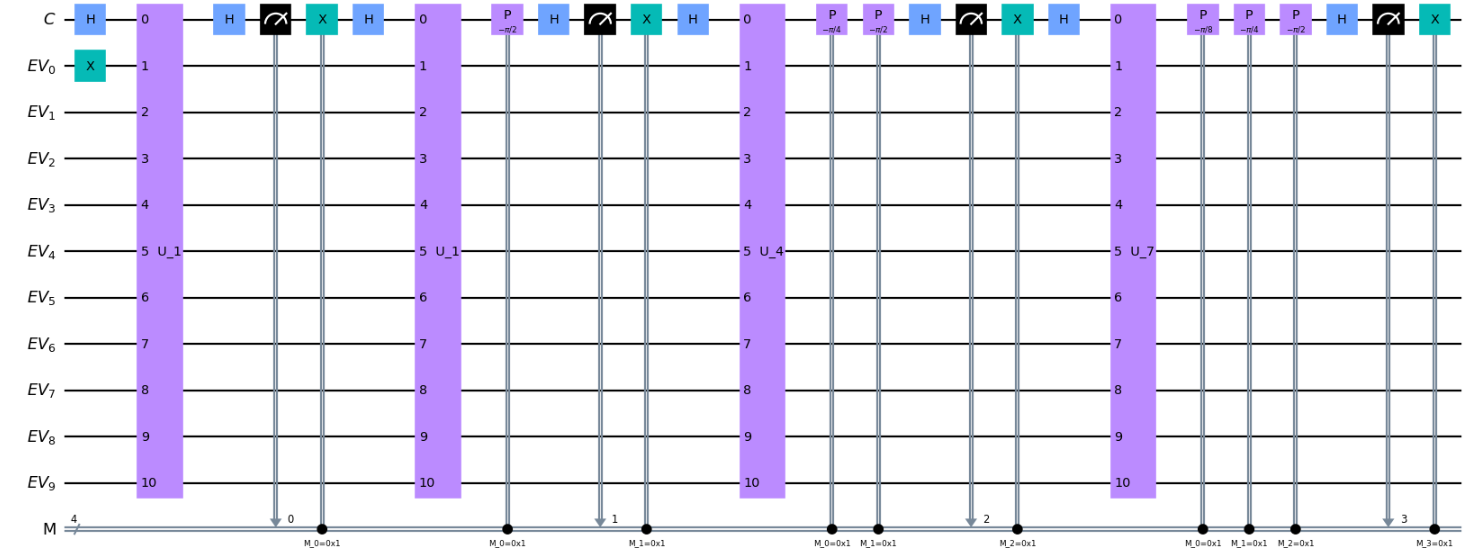
\includegraphics[scale = 0.4]{code_iterative_QPE_qiskit.PNG}
  \caption{iterative QPE Beispiel in qiskit}
  \label{fig:iterative_iQPE_qiskit}
\end{figure}

Der ausschlaggebende Vorteil der iterativen Quantum-Phase-Estimation besteht darin, 
dass diese Variante im Vergleich zur zuvor in Sektion~\ref{section:imp_QPE_Shor} implementierten Variante den Ressourcenbedarf von \(4n+2\) Qubits auf \(2n+3\) Qubits reduziert.

Ein weiterer Vorteil dieser Variante ist, 
dass die Genauigkeit \(k\) nicht auf Kosten von weiteren Qubits erhöht wird, 
sondern ausschließlich durch zusätzliche Gatter.
Deswegen benötigt diese Variante stets \(2n+3\) Qubits, 
sodass der Bedarf an Qubits lediglich von der Größenordnung der Zahl \(N\) abhängig ist.

Der Nachteil der iterativen Variante besteht darin, 
dass die einzelnen Episoden der semi-klassischen Quanten-Fourier-Transformation nicht parallel angewendet werden können.
Hingegen ist es möglich, die regulären inverse Quanten-Fourier-Transformation, bis zu einem gewissen Grad, 
parallel Anzuwenden.
Da dies aber lediglich die letzte Anwendung der Quanten-Fourier-Transformation im Quantum-Phase-Estimation Algorithmus betrifft, 
ist diese zusätzliche Laufzeit vernachlässigbar.

Da sowohl bei der regulären als auch bei der iterativen Variante, 
alle \(U^{2^x}\)-Gatter auf dasselbe Quantenregister wirken, 
können diese nur sequenziell angewendet werden.

Zusammengefasst tauscht man bei der Verwendung der iterativen Variante, 
einen breiteren Quantenschaltkreis gegen einen minimal tieferen ein.

Welche der beiden Varianten vorzuziehen ist, 
hängt vor allem von den zur Verfügung stehenden Ressourcen des Quantencomputers ab.

\bigskip

Die Konstruktion der iterativen Anwendung nach Beauregard ist in Abbildung~\ref{fig:iterative_iQPE_Beauregard} dargestellt.
Anhand der Grafik ist erkennbar, 
dass sowohl die Anwendung der \(U^{2^x}\)-Gatter als auch die Messungen der Qubits in Reihenfolge einer aufsteigenden Wertigkeit geschieht.
Die Anwendung der Gatter und Messungen in dieser Reihenfolge stimmt nicht mit anderen Quellen überein~\cite{Parker2000}.

\begin{figure}[H]
  \centering
  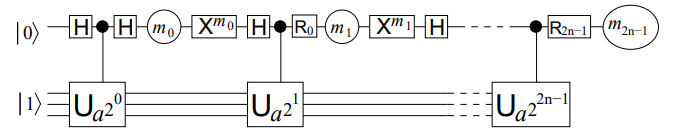
\includegraphics[scale = 0.6]{beauregard_iterative_QPE.png}
  \caption{iterative QPE nach Beauregard~\cite{beauregard2003circuit}}
  \label{fig:iterative_iQPE_Beauregard}
\end{figure}

Wie in Abbildung~\ref{fig:iQFTswaps} für die inverse Quanten-Fourier-Transformation zu sehen ist, 
werden die Gatter auf den Eingangszustand \(\ket{q1}\) durch die Ergebnisse der beiden anderen Kontrollqubits kontrolliert.
Für die iterative Variante nach Beauregard bedeutet das, 
dass die klassisch kontrollierten Phasen-Gatter auf \(\ket{q1}\) von klassischen Bits kontrolliert werden, 
welche noch nicht das Messergebnis beinhalten.
Derselbe Effekt tritt auch für die weiteren Qubits auf.

Ein Nachbau des iterativen Quantenschaltkreises nach Beauregard wie in Abbildung~\ref{fig:iterative_iQPE_Beauregard_qiskit} für \(a = 7,~N=15,~k=4\), 
konnte die Funktionsweise in Simulationen nicht bestätigen.
\begin{figure}[H]
  \centering
  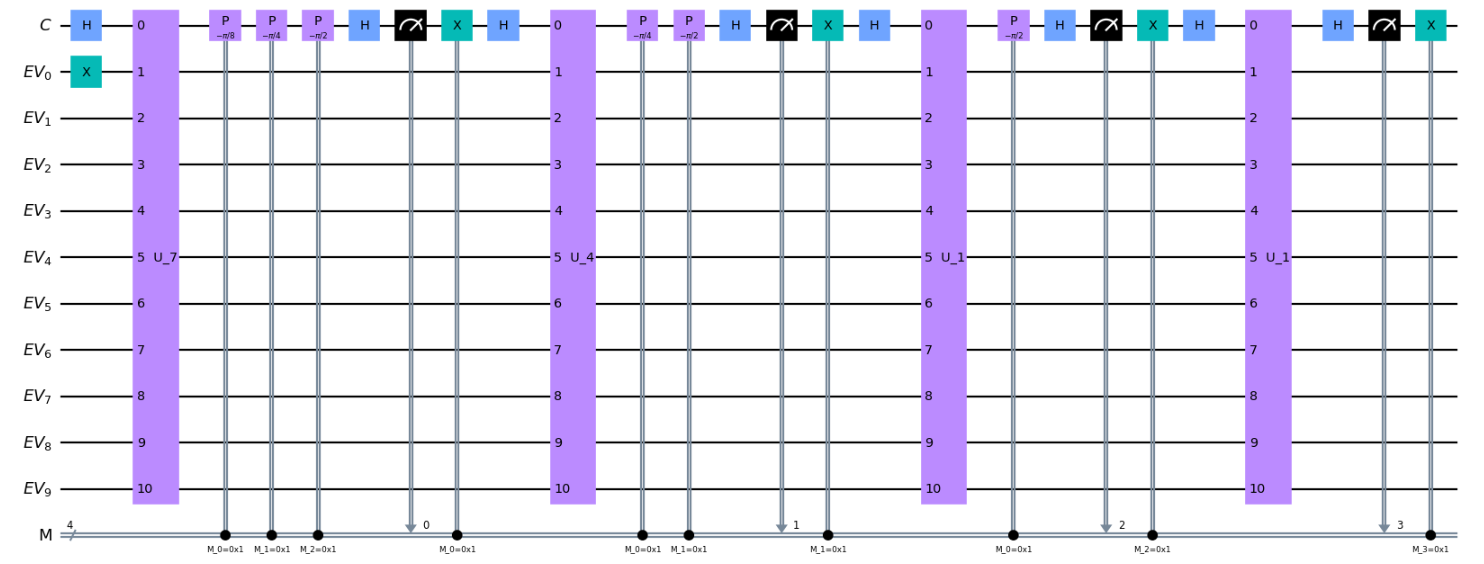
\includegraphics[width=\textwidth]{beauregard_iterative_QPE_qiskit.PNG}
  \caption{iterative QPE Beispiel nach Beauregard}
  \label{fig:iterative_iQPE_Beauregard_qiskit}
\end{figure}
Der Vergleich beider Quantenschaltkreise wird in Abbildung~\ref{fig:iterative_iQPE_Vergleich} dargestellt.
Links sind die Ergebnisse des Quantenschaltkreises aus Abbildung~\ref{fig:iterative_iQPE_qiskit}, 
rechts die des Quantenschaltkreises nach Abbildung~\ref{fig:iterative_iQPE_Beauregard_qiskit}.
Beide Quantenschaltkreise sind für \(a = 7,~N=15,~k=4\) nachgebildet.
Lediglich das Ergebnis auf der linken Seite ist korrekt, 
da die Messergebnisse übereinstimmen, 
als auch genau vier Peaks vorhanden sind, 
was der Länge der Periode entspricht.
\begin{figure}[H]
  \centering
  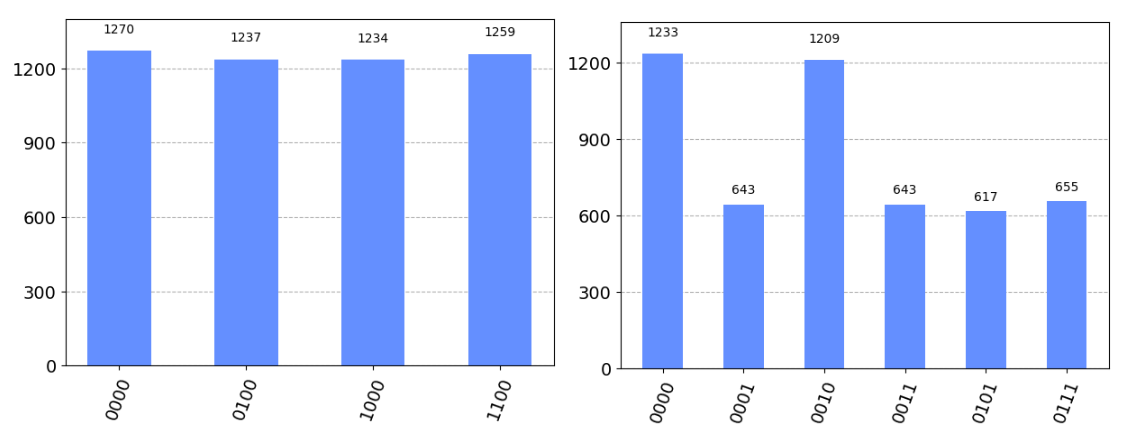
\includegraphics[scale = 0.4]{Vergleich_interative_QPE.png}
  \caption{iterative QPE Messergebnisse(Beauregard rechts)}
  \label{fig:iterative_iQPE_Vergleich}
\end{figure}

Um ein Missverständnis auszuschließen, wurde versucht, Stéphane Beauregard zu kontaktieren. 
Leider waren keine Kontaktinformationen auf den Portalen hinterlegt, 
auf denen seine Arbeiten öffentlich zugänglich sind. 
Die einzige nützliche Information, die dabei gefunden wurde, 
war seine Zugehörigkeit zur University of Montreal. 
Auf LinkedIn wurde ein anderer Stéphane Beauregard gefunden, 
der zufällig auch an der University of Montreal war. Auf Nachfrage wurde jedoch herausgefunden, 
dass es sich um eine andere Person handelt. 
Eine Anfrage bei der University of Montreal selbst war aus Datenschutzgründen erfolglos. 
Als letzte Option wurde der häufigste Co-Autor kontaktiert. 
Der Co-Autor Guy Lapalme ist emeritierter Professor der University of Montreal.
Da Beauregard die University of Montreal verlassen hat, 
hatte auch Guy Lapalme keine Kontaktinformationen von Beauregard.

\bigskip

Im Faktorisierungsalgorithmus wird die iterative Quantum-Phase-Estimation genutzt, 
wenn die Anzahl der erforderlichen Qubits für die reguläre Variante mit \(4n+2\) Qubits einen zu hohen Ressourcenbedarf darstellt, 
den der genutzte Quantencomputer nicht bereitstellen kann. 
In diesem Fall wird auf Kosten der Laufzeit die sparsamere Variante angewendet. 
Sollten auch dafür nicht genügend Qubits vorhanden sein, 
wird die Berechnung mit einer Fehlermeldung abgebrochen. 
Die Fallunterscheidung in der Implementierung wird realisiert, 
indem statt der Funktion \texttt{Shor} die iterative Variante \texttt{Shor\_sequential} ausgeführt wird. 
Weitere Anpassungen sind nicht nötig, 
da sowohl die Eingabewerte als auch die Form der Rückgabewerte identisch sind.

\subsubsection{Approximative Quanten-Fourier-Transformation} \label{sec:ApproxQFT}
Die zweite Methode zur Ressourceneinsparung betrifft ebenfalls die Quanten-Fourier-Transformation und 
wurde erstmals 1996 vorgestellt~\cite{Barenco_1996}.
Bei dieser Optimierung wird die Ressourceneffizienz durch die Reduktion der verwendeten Gatter erreicht. 
Sowohl die reguläre als auch die iterative Quanten-Fourier-Transformation verwenden (klassisch) kontrollierte Phasen-Gatter.
Dabei kommen Phasenverschiebungen im Bereich von \(e^{\frac{2\pi i}{2^1}}\) bis \(e^{\frac{2\pi i}{2^n}}\) zur Anwendung. 
Dies führt zu einem exponentiellen Wachstum der Zweierpotenz im Nenner des Bruchs der wirkenden Phasenverschiebung, 
was wiederum eine exponentielle Abnahme der wirkenden Phasenverschiebungen bei jedem weiteren Phasen-Gatter bewirkt. 

Die approximative Quanten-Fourier-Transformation nutzt den Effekt aus, 
dass die Beiträge höherer Phasen-Gatter für das Endergebnis oft weniger kritisch sind, 
um eine reduzierte Anzahl an Gattern einzusetzen. 
Indem ein angemessener Approximationsfaktor gewählt wird, 
kann eine Genauigkeit erzielt werden, 
die weiterhin für ein akzeptables Endergebnis ausreichend ist.

Die approximative Quanten-Fourier-Transformation wird als \(AQFT_m\) definiert und 
wendet maximal \(m\) Phase-Gatter pro Qubit an. 
Der Parameter \(m\) wird als Approximationsfaktor bezeichnet und bestimmt die Präzision der \(AQFT_m\). 
Der Approximationsfaktor gibt an, 
bis zu welcher Phasenverschiebung von \(e^{\frac{2\pi i}{2^m}}\) die Phasen-Gatter angewendet werden.
Die vollständige Quanten-Fourier-Transformation entspricht einer \(AQFT_n\).

Wenn der Approximationsfaktor \(m\) einen Wert
\[m \geq \ld(n)+2\]
entspricht, nähert sich die Wahrscheinlichkeit, das optimale Ergebnis mit \(AQFT_m\)
zu erhalten, dem Wert~\cite{cheung2004improved}: 
\[P \geq \frac{4}{\pi^2} - \frac{1}{4n}\]
Dies steht im Gegensatz zur Wahrscheinlichkeit von \(\frac{4}{\pi^2}\), 
die für die exakte Quanten-Fourier-Transformation \(QFT\) gilt~\cite{cheung2004improved}\cite[119]{kaye2007introduction}.

Im Hinblick auf die Ressourceneffizienz benötigt die \(AQFT_m\) insgesamt \(\Landau(nm)\) Gatter.
Wenn \(m\) wie zuvor definiert wird, entspricht dies \(\Landau(n~\ld(n))\). 
Im Vergleich dazu erfordert die exakte Quanten-Fourier-Transformation \(\Landau(n^2)\) Gatter~\cite{Barenco_1996}.
Die Tiefe der Schaltung wird durch die approximative Quanten-Fourier-Transformation im Vergleich zur exakten nicht verändert.

Daraus folgt, dass die approximative Quanten-Fourier-Transformation einen effizienteren Bedarf an Gattern aufweist, 
jedoch zulasten einer geringeren Genauigkeit im Vergleich zur exakten Quanten-Fourier-Transformation.
Aufgrund der identischen Tiefe beider Varianten ist die Laufzeit beider Varianten ebenfalls identisch.

Allerdings gilt dies nur unter der Annahme, 
dass der Quantencomputer ideal ist und weder Dekohärenzeffekte noch andere Fehler aufweist.
Im Falle eines idealen Quantencomputers liefert die exakte Quanten-Fourier-Transformation, die alle Phasen-Gatter anwendet, 
mit höherer Wahrscheinlichkeit ein genaues Ergebnis als die approximative Quanten-Fourier-Transformation.

Wenn allerdings kein idealer Quantencomputer genutzt wird, 
führt die Dekohärenz, 
bedingt durch eine Vielzahl an Gattern, 
zu einer erhöhten Fehlerrate.
Eine Reduktion der Anzahl an Gattern durch ein geringeres 
\(m\) führt daher zu einer niedrigeren Fehlerrate durch Dekohärenz, 
was wiederum die Wahrscheinlichkeit für ein genaues Ergebnis erhöht.
Auf der anderen Seite führt ein geringeres \(m\) zu einer Ungenauigkeit,
da der Approximationsfaktor größer ist und somit nicht alle Phasen-Gatter angewendet werden.
Um das bestmögliche Ergebnis zu erzielen, 
muss eine gewisse Ungenauigkeit durch die Approximation in Kauf genommen werden, 
die wiederum durch die geringere Fehlerrate kompensiert wird. 
Das optimale \(m\) nähert sich der Untergrenze von~\cite{Barenco_1996}:
\[m \geq \ld(n)+2\]

Die Approximationstechnik kann auch in der iterativen beziehungsweise, 
semi"=klassisch\-en Quanten-Fourier-Transformation angewendet werden. 
Bei der Implementierung für den Shor-Algorithmus ist darauf zu achten, 
dass alle verwendeten Quanten"=Fourier"=Transformationen, also sowohl die in den \(U^{2^x}\)-Gattern als auch die finale Transformation vor dem Basiswechsel, 
das gleiche \(m\) nutzen.
Andernfalls wären die angewendeten und extrahierten Phasenverschiebungen inkonsistent 
und würden zu falschen Ergebnissen führen.

Die Implementierung des \texttt{Faktorisierungsalgorithmus} wird um den Parameter \(m\) ergänzt.
Standardmäßig entspricht der Approximationsfaktor 
\[m = \lceil\ld(n)+2\rceil\]  
Dieser kann jedoch über den Parameter beliebig angepasst oder 
durch Setzen von \(m=-1\) deaktiviert werden.
Im Falle der Deaktivierung wird die exakte Quanten-Fourier-Transformation angewendet.

Der Grund, warum die approximative Variante standardmäßigen verwendet wird, 
liegt darin, dass das Ergebnis bereits bei kleinen \(n\) eine gute Genauigkeit gewährt. 
Dies wird deutlich, wenn man Abbildung~\ref{fig:shor_measure} mit \(m=n=7\) und
Abbildung~\ref{fig:shor_measure_AQFT} mit \(m=4\) vergleicht.
Abgesehen von \(m\) sind die Berechnungen in beiden Abbildungen identisch.
Mit steigendem \(n\) nimmt die Ungenauigkeit durch die fehlenden Gatter ab, 
bis sie schließlich ganz vernachlässigbar wird~\cite{cheung2004improved}.

\begin{figure}[H]
  \centering
  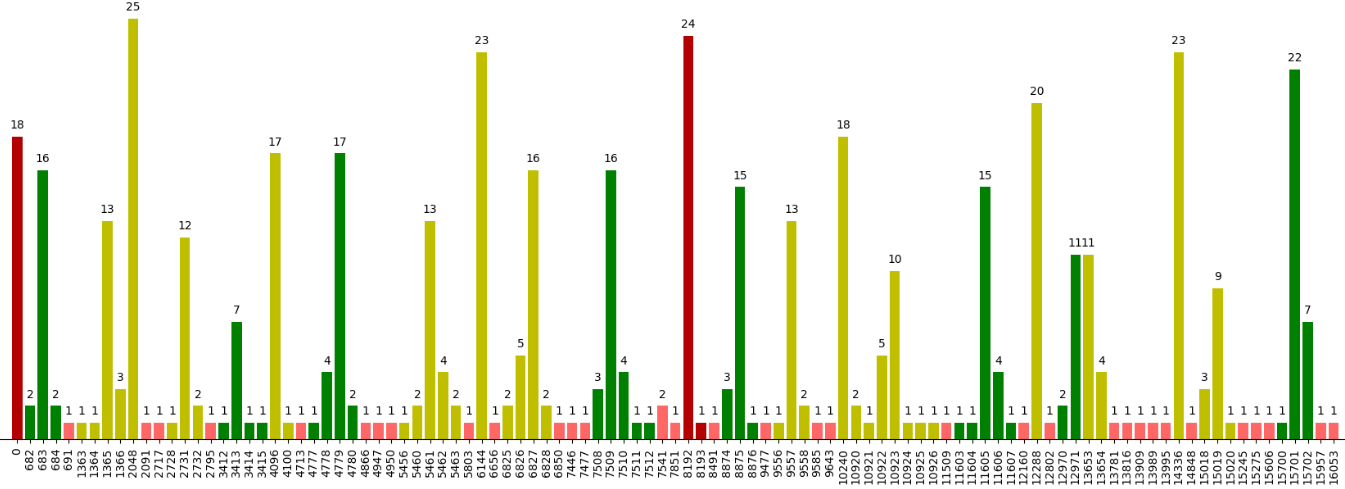
\includegraphics[width=\textwidth]{shor_measure_AQFT.PNG}
  \caption{AQFT Messung a=19, N=119, k=14, m=4}
  \label{fig:shor_measure_AQFT}
\end{figure}
